% =====================================================================
%  Ponencia - X Encuentro Regional & I Congreso Internacional de Ciencias Físicas
%  S. Gaviria Giraldo, D. J. Duque Tamayo, O. L. López Acevedo, H. D. Salinas Jiménez
%  "Estudio del crecimiento de cristales de hemozoína (beta-hematina) en
%   Plasmodium falciparum mediante un modelo de Monte Carlo cinético"
%  Trabajo de grado, Instituto de Física, Universidad de Antioquia (2026)
%  Compilar con: pdflatex slides.tex  o bien  tectonic slides.tex
% =====================================================================
\documentclass[aspectratio=169,11pt]{beamer}

\usepackage{iftex}
\ifPDFTeX
  \usepackage[T1]{fontenc}
  \usepackage[utf8]{inputenc}
  \usepackage{lmodern}
\fi
\usepackage[spanish,es-nodecimaldot,es-noshorthands]{babel}
\usepackage{amsmath,amssymb}
\usepackage{graphicx}
\usepackage{grffile}
\usepackage{booktabs}
\usepackage{array}
\usepackage{tikz}
\usepackage{appendixnumberbeamer}
\usetikzlibrary{arrows.meta,positioning,calc}
\graphicspath{{../figures/}{./}}

% ---------------------------------------------------------------------
%  Paleta de colores oficial del congreso y compatibilidad
% ---------------------------------------------------------------------
\definecolor{FisicaAzulOscuro}{RGB}{11, 60, 104}
\definecolor{FisicaCyan}{RGB}{0, 140, 185}
\definecolor{FisicaVerde}{RGB}{46, 139, 87}
\definecolor{TextoPrincipal}{RGB}{30, 41, 59}
\definecolor{gris}{RGB}{100, 110, 125}
\definecolor{acento}{RGB}{190, 45, 45}

% Mapeo de compatibilidad con estilos y figuras TikZ existentes
\colorlet{azul}{FisicaAzulOscuro}
\colorlet{azulclaro}{FisicaCyan!10}

\usefonttheme{professionalfonts}
\setbeamertemplate{navigation symbols}{}

% --- Configuración de elementos en Beamer ---
\setbeamercolor{normal text}{fg=TextoPrincipal}
\setbeamercolor{structure}{fg=FisicaAzulOscuro}
\setbeamercolor{frametitle}{fg=FisicaAzulOscuro}
\setbeamercolor{framesubtitle}{fg=FisicaCyan}
\setbeamercolor{title}{fg=FisicaAzulOscuro}
\setbeamercolor{subtitle}{fg=FisicaCyan}
\setbeamercolor{author}{fg=TextoPrincipal}
\setbeamercolor{institute}{fg=TextoPrincipal!80}
\setbeamercolor{date}{fg=TextoPrincipal!70}

% Configuración de bloques temáticos
\setbeamercolor{block title}{bg=FisicaAzulOscuro, fg=white}
\setbeamercolor{block body}{bg=FisicaAzulOscuro!6, fg=TextoPrincipal}
\setbeamercolor{block title example}{bg=FisicaCyan, fg=white}
\setbeamercolor{block body example}{bg=FisicaCyan!6, fg=TextoPrincipal}
\setbeamertemplate{blocks}[rounded][shadow=false]

% Viñetas y listas
\setbeamercolor{item}{fg=FisicaCyan}
\setbeamercolor{subitem}{fg=FisicaAzulOscuro}
\setbeamertemplate{itemize items}{\small$\blacktriangleright$}

% Tipografías
\setbeamerfont{frametitle}{series=\bfseries, size=\large}
\setbeamerfont{framesubtitle}{series=\normalfont, size=\small}
\setbeamerfont{caption}{size=\scriptsize}
\setbeamertemplate{caption}{\raggedright\insertcaption\par}

% --- Fondo con imagen del congreso y logo institucional ---
\setbeamertemplate{background}{%
  
\includegraphics[width=\paperwidth,height=\paperheight]{fondo_pptx.jpg}%
  \begin{tikzpicture}[remember picture,overlay]
    \ifnum\value{page}=1
      % Portada: logo institucional en la esquina inferior izquierda (más grande)
      \node[anchor=south west,inner sep=0pt,xshift=0.1cm,yshift=0.85cm] at (current page.south west) {%
        \includegraphics[height=1.25cm]{"lOGO png.png"}%
      };
    \else
      % Resto de diapositivas: logo compacto que no interfiere con el contenido
      \node[anchor=south west,inner sep=0pt,xshift=0.1cm,yshift=0.85cm] at (current page.south west) {%
        \includegraphics[height=0.5cm]{"lOGO png.png"}%
      };
    \fi
  \end{tikzpicture}%
}

% =====================================================================
%  CONTROL DE ZONAS SEGURAS (MÁRGENES, ENCABEZADO Y PIE DE PÁGINA)
% =====================================================================

% Fondo 1376x768 px sobre 16x9 cm (86 px/cm): banner superior hasta 1.36 cm,
% barra inferior desde 0.83 cm del borde. El logo compacto (0.5 cm de alto,
% ~1.3 cm de ancho) vive dentro del margen izquierdo, así que los márgenes
% laterales son simétricos y el contenido queda centrado en la zona blanca.

% 1. ENCABEZADO: despeja el banner superior (1.36 cm) con un respiro
\setbeamertemplate{headline}{%
  \vspace{1.45cm}%
}

% 2. PIE DE PÁGINA: despeja la barra inferior (0.83 cm) con un respiro
\setbeamertemplate{footline}{%
  \vspace{1.0cm}%
}

% 3. MÁRGENES LATERALES simétricos (el logo cabe en el izquierdo)
\setbeamersize{text margin left=1.45cm, text margin right=1.45cm}

% 4. TÍTULO DE LA DIAPOSITIVA (frametitle limpio sobre el fondo blanco)
\makeatletter
\setbeamertemplate{frametitle}{%
  \nointerlineskip%
  \begin{beamercolorbox}[wd=\linewidth,left]{frametitle}%
    {\usebeamerfont{frametitle}\insertframetitle}%
    \hskip 0pt plus 1filll%
    {\footnotesize\color{FisicaCyan}\textbf{\insertframenumber\,/\,\inserttotalframenumber}}\par%
    \ifx\insertframesubtitle\@empty\else%
      \vspace{0.05cm}%
      {\usebeamerfont{framesubtitle}\usebeamercolor[fg]{framesubtitle}\insertframesubtitle\par}%
    \fi%
  \end{beamercolorbox}%
  \vspace{0.12cm}%
}
\makeatother

% --- Comandos y utilidades ---
\newcommand{\kB}{k_{B}}
\newcommand{\fig}[1]{{\scriptsize\color{gris}#1}}
\newcommand{\snap}[2]{\includegraphics[height=#1,trim=18 39 3 72,clip]{#2}}

% --- Estilos TikZ adaptados a la nueva paleta ---
\tikzset{
  cab/.style={fill=azul,text=white,rounded corners=3pt,font=\small\bfseries,
              text width=3.8cm,align=center,inner sep=3pt,minimum height=0.6cm},
  caja/.style={draw=azul,fill=azulclaro,rounded corners=3pt,font=\footnotesize,
               text width=3.8cm,align=flush left,inner sep=5pt,anchor=north},
  paso/.style={-{Stealth},very thick,acento},
  etapa/.style={draw=azul,fill=azulclaro,rounded corners=3pt,font=\footnotesize,
                align=center,inner sep=4pt},
}

% ---------------------------------------------------------------------
\title[kMC para hemozoína]{Estudio del crecimiento de cristales de hemozoína
  ($\beta$-hematina) en \textit{Plasmodium falciparum} mediante un modelo de
  Monte Carlo cinético}
\author{S.~Gaviria~Giraldo \and D.~J.~Duque~Tamayo \and O.~L.~López~Acevedo \and H.~D.~Salinas~Jiménez}
\institute{Instituto de Física, Universidad de Antioquia}
% =====================================================================

\begin{document}

% ---------------------------------------------------------------- 1: Portada
\begin{frame}
  \vspace{0.1cm}
  \begin{center}
    {\Large\bfseries\color{FisicaAzulOscuro} Estudio del crecimiento de cristales de hemozoína\\[0.15em]
    ($\beta$-hematina) en \textit{Plasmodium falciparum} mediante un\\[0.15em]
    modelo de Monte Carlo cinético}\\[0.25cm]
    {\color{FisicaCyan}\rule{0.45\linewidth}{1.2pt}}\\[0.35cm]
    
    {\normalsize \textbf{S.~Gaviria~Giraldo},\; \textbf{D.~J.~Duque~Tamayo},\; O.~L.~López~Acevedo,\; H.~D.~Salinas~Jiménez}\\[0.25cm]
    {\footnotesize\color{TextoPrincipal!80} Instituto de Física, Facultad de Ciencias Exactas y Naturales\\
     Universidad de Antioquia, Medellín, Colombia}\\[0.35cm]

  \end{center}
\end{frame}

% ---------------------------------------------------------------- 2: Contexto
\begin{frame}{La malaria: un problema vigente}{Para sobrevivir, el parásito cristaliza el hemo tóxico en hemozoína: un blanco farmacológico.}
  \begin{columns}[c,onlytextwidth]
    \begin{column}{0.52\textwidth}
      \centering
      \renewcommand{\arraystretch}{1.25}
      \begin{tabular}{@{}r@{\hspace{0.5em}}l@{}}
        {\Large\bfseries\color{azul}282\,M} & casos de malaria (2024) \\
        {\Large\bfseries\color{azul}610\,000} & muertes, 80 países endémicos \\
        {\Large\bfseries\color{acento}$\sim$95\,\%} & de las muertes: \textit{P.~falciparum} \\
      \end{tabular}\\[0.4em]
      \begin{block}{Resistencia farmacológica}
        \scriptsize Resistencia parcial a derivados de \textbf{artemisinina}
        (Gran Mekong y África) $\Rightarrow$ urge entender los mecanismos de supervivencia del parásito.
      \end{block}
      \fig{World Health Organization, \textit{World malaria report} (2025).}
    \end{column}
    \begin{column}{0.46\textwidth}
      \centering
      \begin{tikzpicture}[node distance=0.30cm,
          e/.style={etapa,text width=3.7cm}]
        \node[e] (hb) {\textbf{Hemoglobina} del eritrocito};
        \node[e,below=of hb] (hemo) {\textbf{Hemo libre}, Fe(II)};
        \node[e,below=of hemo,draw=acento,fill=acento!10] (fp) {\textbf{Fe(III)-protoporfirina IX}\\ {\scriptsize tóxica para el parásito}};
        \node[e,below=of fp,fill=azul,text=white] (hz) {\textbf{Hemozoína} (cristal inerte)};
        \draw[paso] (hb) -- node[right,font=\scriptsize,gris]{digestión (vacuola)} (hemo);
        \draw[paso] (hemo) -- node[right,font=\scriptsize,gris]{oxidación} (fp);
        \draw[paso] (fp) -- node[right,font=\scriptsize,gris]{cristalización} (hz);
        \node[font=\scriptsize\bfseries,acento,anchor=east] at ([xshift=-0.12cm]$(fp.west)!0.5!(hz.west)$) {¿inhibir?};
      \end{tikzpicture}
    \end{column}
  \end{columns}
\end{frame}

% ---------------------------------------------------------------- 3: Hipótesis
\begin{frame}{Hipótesis y objetivo}
  \begin{columns}[T,onlytextwidth]
    \begin{column}{0.485\textwidth}
      \begin{block}{Hipótesis}
        \small Desde la física estadística se puede implementar un modelo de
        \textbf{Monte Carlo cinético} (kMC) que reproduzca la \textbf{cinética} y la
        \textbf{morfología superficial} del crecimiento de cristales de hemozoína
        ($\beta$-hematina).
      \end{block}
    \end{column}
    \begin{column}{0.485\textwidth}
      \begin{block}{Objetivo general}
        \small Diseñar, implementar y validar computacionalmente un modelo kMC
        \textbf{3D} (SOS), que reproduzca la cinética y morfología
        del crecimiento de cristales de hemozoína.
      \end{block}
    \end{column}
  \end{columns}
  \vspace{0.8em}
  \centering
  \begin{tikzpicture}[node distance=0.26cm,
      s/.style={etapa,text width=2.0cm,minimum height=1.15cm}]
    \node[s] (a) {Estructura de la $\beta$-hematina\\ {\scriptsize UC $\pi$--$\pi$}};
    \node[s,right=of a] (b) {Energías $E_{pb}$\\ {\scriptsize MACE-POLAR}};
    \node[s,right=of b] (c) {Nucleación 2D y cinética};
    \node[s,right=of c] (d) {Modelo kMC 3D\\ {\scriptsize eventos y tasas}};
    \node[s,right=of d,fill=azul,text=white] (e) {Cinética y morfología superficial};
    \foreach \i/\j in {a/b,b/c,c/d,d/e} \draw[paso] (\i) -- (\j);
    \draw[->,thick,acento] ([yshift=-0.3cm]a.south west) -- ([yshift=-0.3cm]e.south east);
    \node[font=\scriptsize,gris,anchor=north west] at ([yshift=-0.35cm]a.south west) {microscópico};
    \node[font=\scriptsize,gris,anchor=north east] at ([yshift=-0.35cm]e.south east) {mesoscópico};
  \end{tikzpicture}
\end{frame}

% ---------------------------------------------------------------- 4: Estructura
% \begin{frame}{Estructura de la $\beta$-hematina}
%   \framesubtitle{Unidad de crecimiento (UC) = dímero $\pi$--$\pi$; el cristal se ensambla por niveles.}
%   \begin{columns}[c,onlytextwidth]
%     \begin{column}{0.23\textwidth}
%       \centering
%       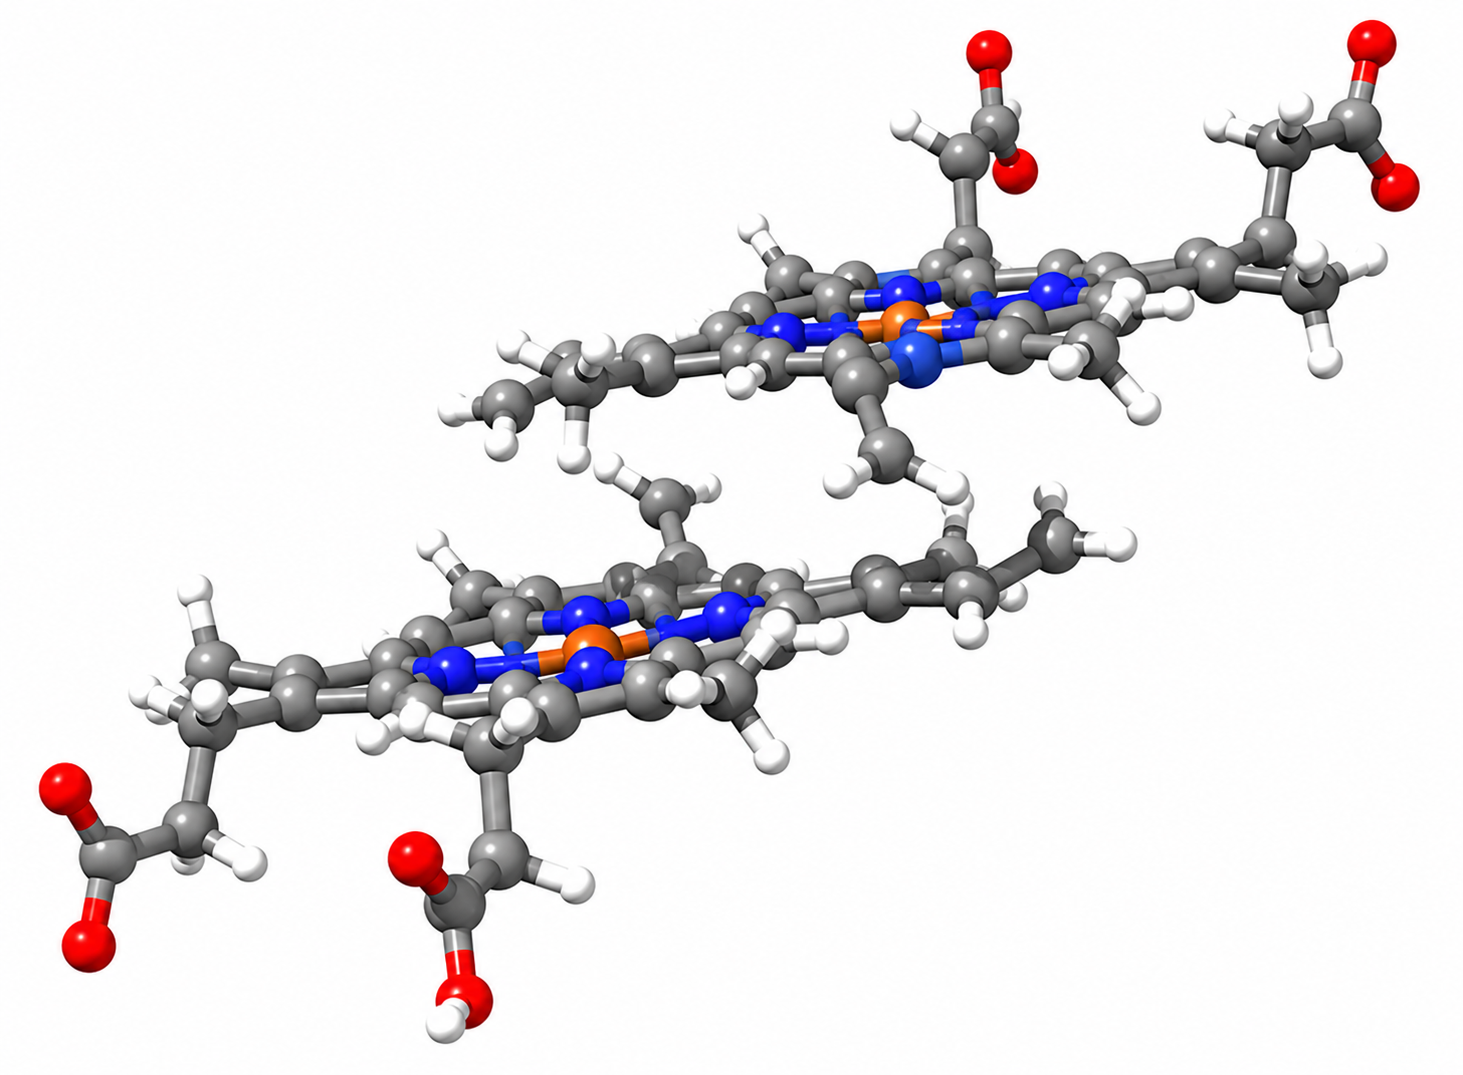
\includegraphics[width=\linewidth]{GU_pp.png}\\
%       {\color{azul}\bfseries\small Dímero $\pi$--$\pi$ (UC)}\\[0.2em]
%       {\scriptsize más estable en medio acuoso;\\ candidato a nucleante inicial\\[0.2em]
%        {\color{gris}Klonis \emph{et al.} (2010);\\ Ma \emph{et al.} (2025)}}
%     \end{column}
%     \begin{column}{0.28\textwidth}
%       \centering
%       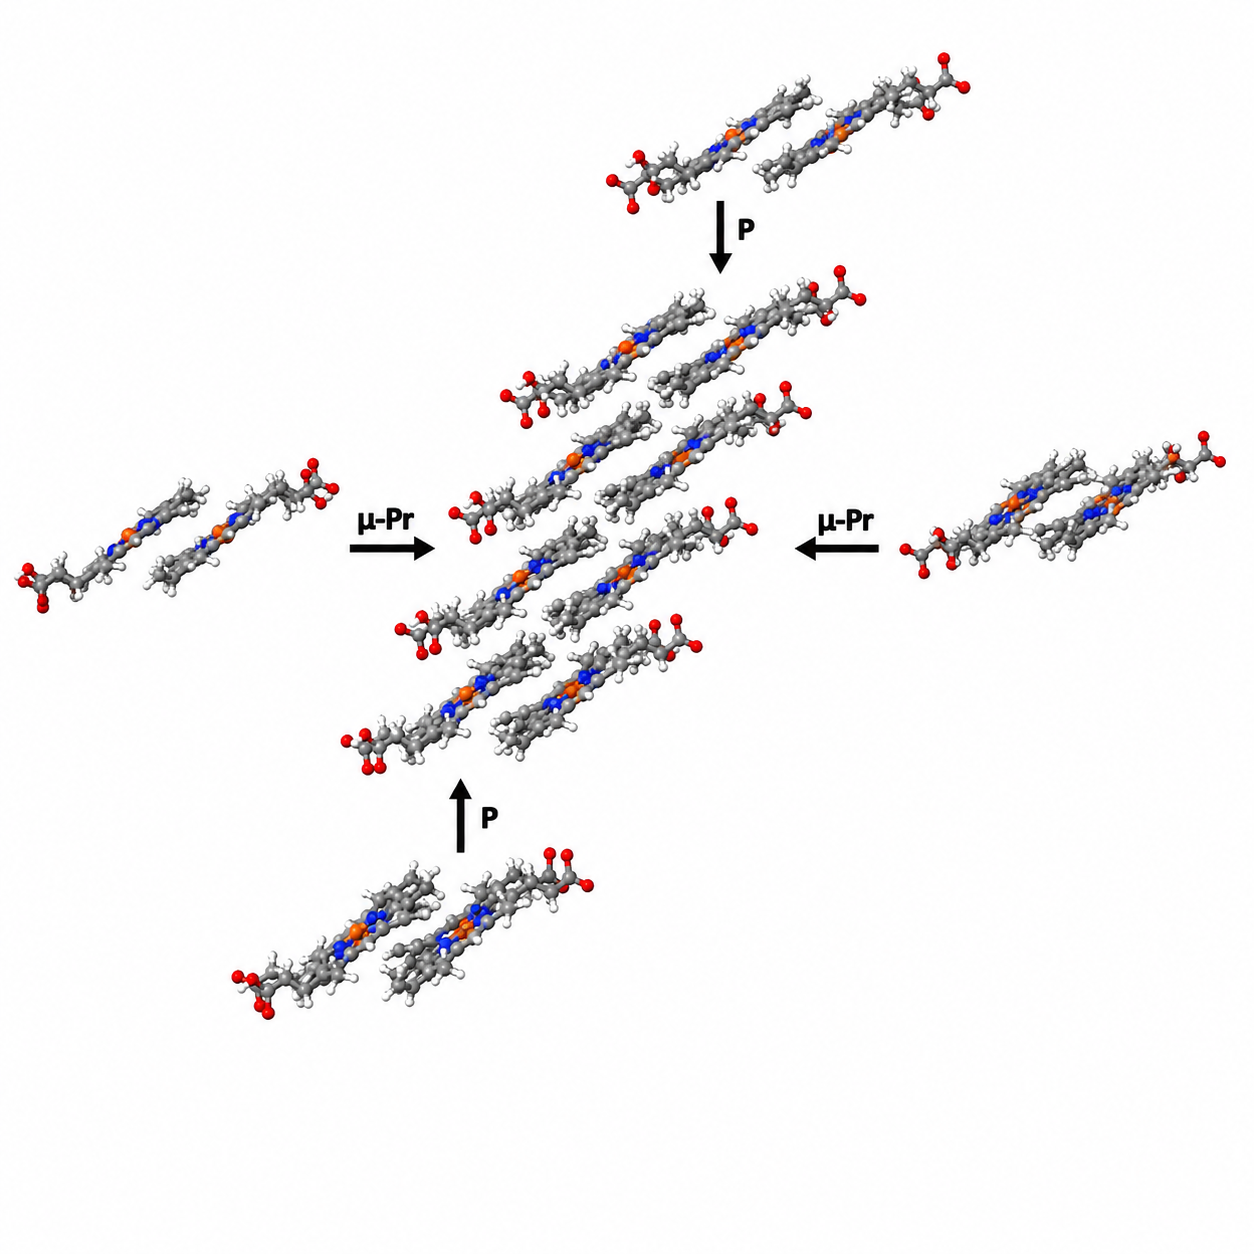
\includegraphics[width=0.95\linewidth]{laywe.png}\\
%       \fig{Fig.~1. Dímeros $\pi$--$\pi$ $\to$ columnas (tipo P) $\to$ láminas 2D ($\mu$-Pr).}
%     \end{column}
%     \begin{column}{0.46\textwidth}
%       \centering
%       \footnotesize
%       \renewcommand{\arraystretch}{1.15}
%       \begin{tabular}{@{}l>{\raggedright\arraybackslash}p{0.55\linewidth}@{}}
%         \toprule
%         Etapa & Interacción \\
%         \midrule
%         \textbf{Nucleación} & dímeros $\pi$--$\pi$ \\
%         \textbf{1D}         & columnas por interacción \textbf{tipo P} \\
%         \textbf{2D}         & láminas por enlaces \textbf{$\mu$-Pr} \\
%         \textbf{3D}         & apilamiento: van der Waals + \textbf{puentes de H} \\
%         \bottomrule
%       \end{tabular}\\[0.5em]
%       \begin{tabular}{@{}c@{\hspace{4pt}}c@{\hspace{4pt}}c@{}}
%         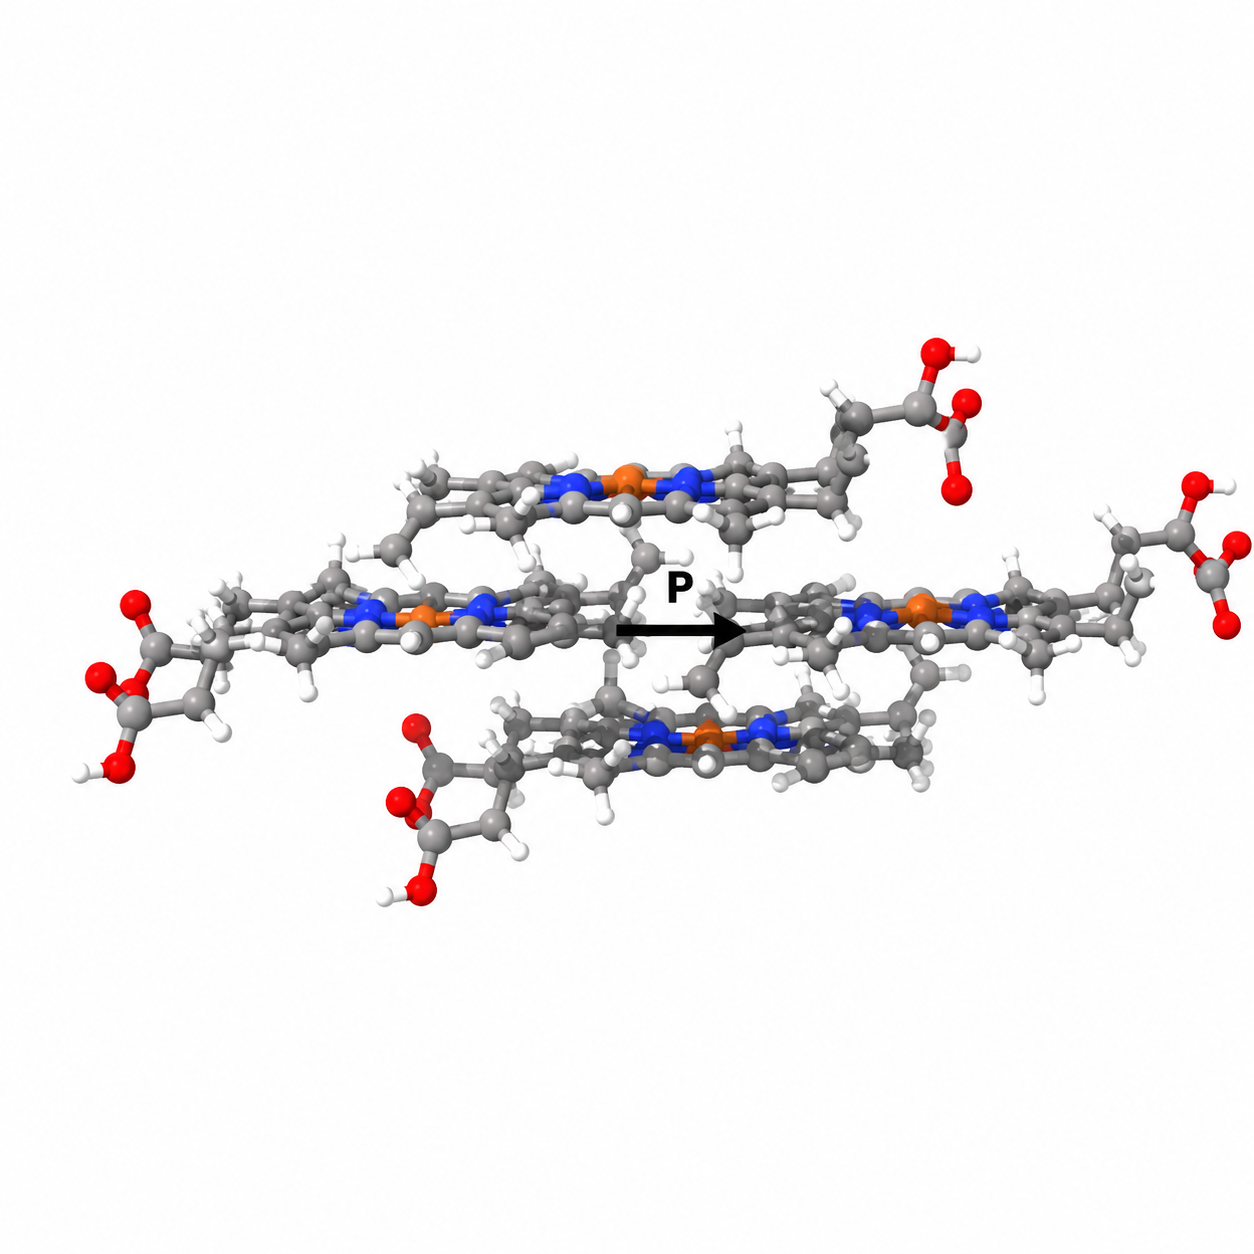
\includegraphics[width=0.25\linewidth,trim=0 60 0 60,clip]{Ptype.png} &
%         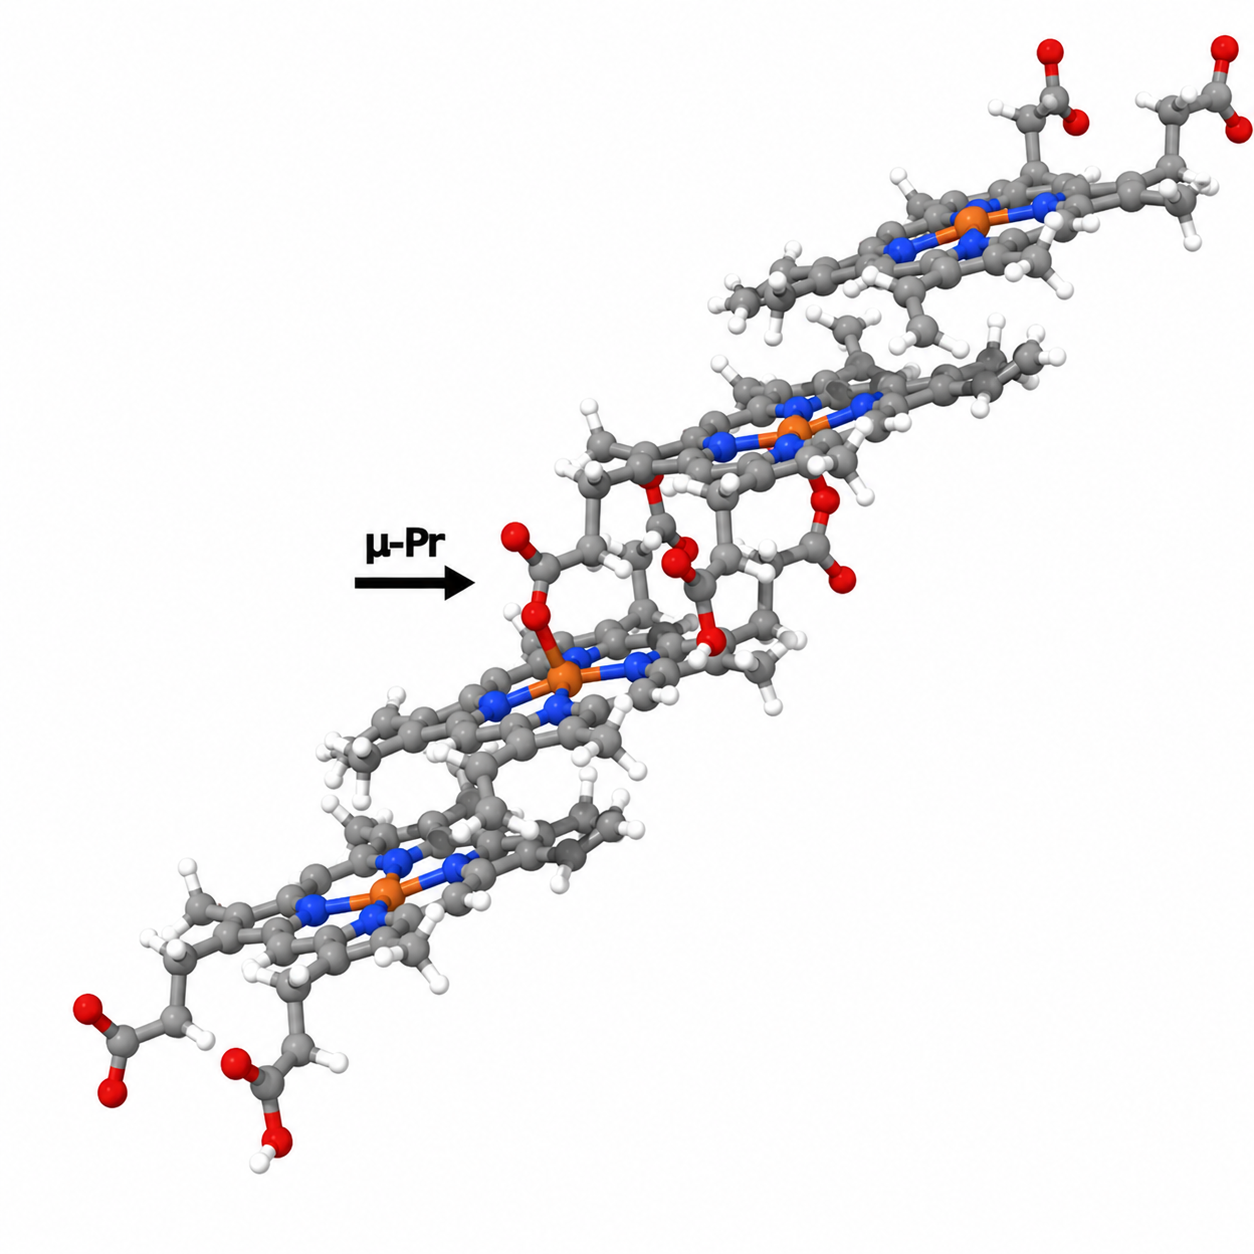
\includegraphics[width=0.25\linewidth,trim=0 60 0 60,clip]{mPr.png} &
%         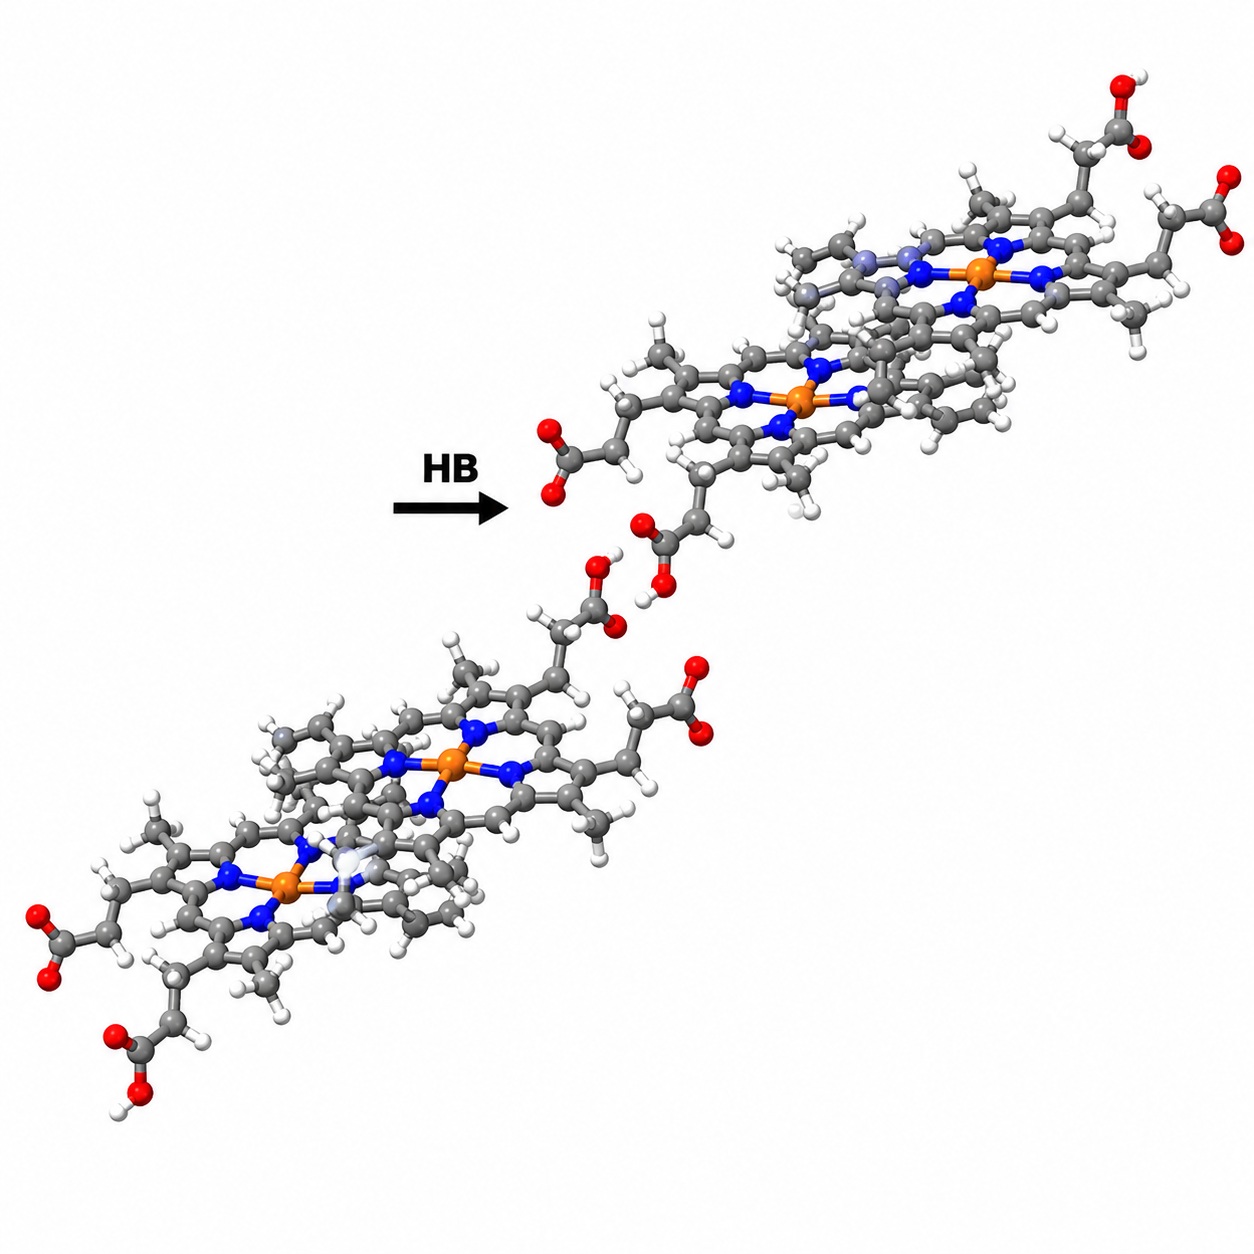
\includegraphics[width=0.25\linewidth,trim=0 60 0 60,clip]{HB.png} \\
%         {\scriptsize tipo P} & {\scriptsize $\mu$-Pr} & {\scriptsize puente de H}
%       \end{tabular}\\[0.2em]
%       {\footnotesize Láminas de grosor $\approx 11$\,\AA}
%     \end{column}
%   \end{columns}
% \end{frame}

% =====================================================================
%  DIAPOSITIVA 1: Unidades de Crecimiento (GU)
% =====================================================================
\begin{frame}{Modelos de la Unidad de Crecimiento (GU)}
  \framesubtitle{Comparación entre los dos candidatos a bloque fundamental de ensamblaje.}
  \begin{columns}[c,onlytextwidth]
    % ---- GU mu-Pr ----
    \begin{column}{0.47\textwidth}
      \centering
      % Ajusta la ruta a "imagenes/GU_mPr.png" o "GU_mPr.png" según tu estructura
      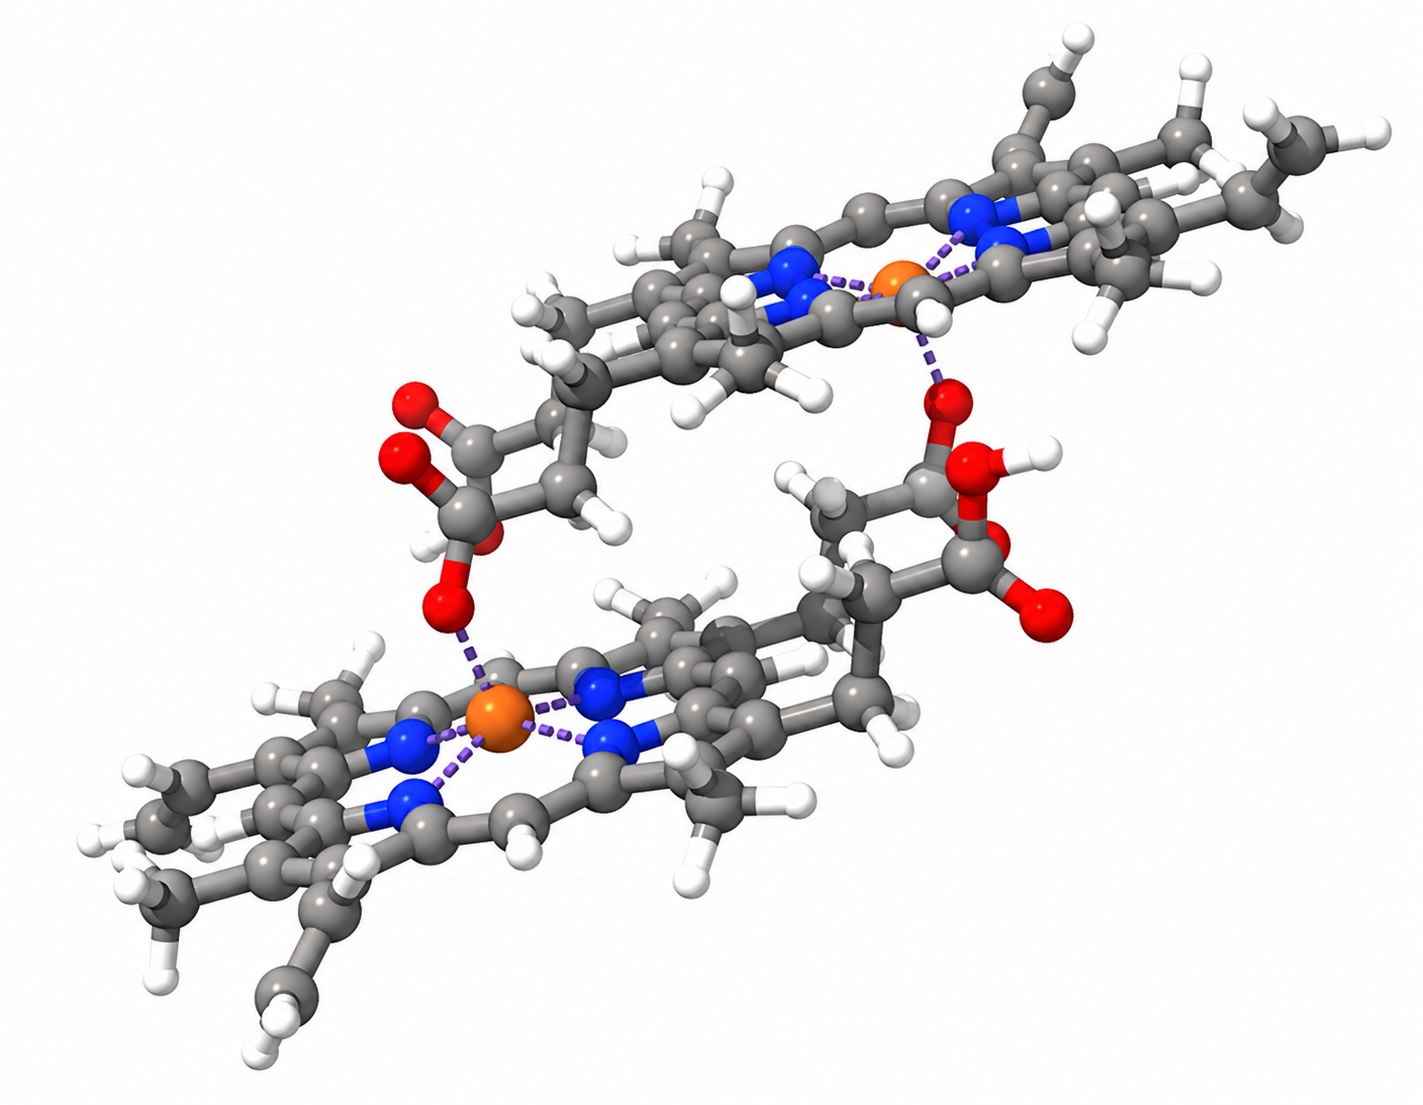
\includegraphics[height=0.55\textheight,keepaspectratio]{GU_mPr.png}\\[0.5em]
      {\color{azul}\bfseries\small (a) Enlaces $\mu$-propionato ($\mu$-Pr)}\\[0.2em]
      {\footnotesize Coordinación Fe--carboxilato entre dímeros. \\
      {\scriptsize\color{gris}Pagola \emph{et al.} (2000); Becker \emph{et al.} (2016)}}
      
    \end{column}

    % ---- GU pi-pi ----
    \begin{column}{0.47\textwidth}
      \centering
      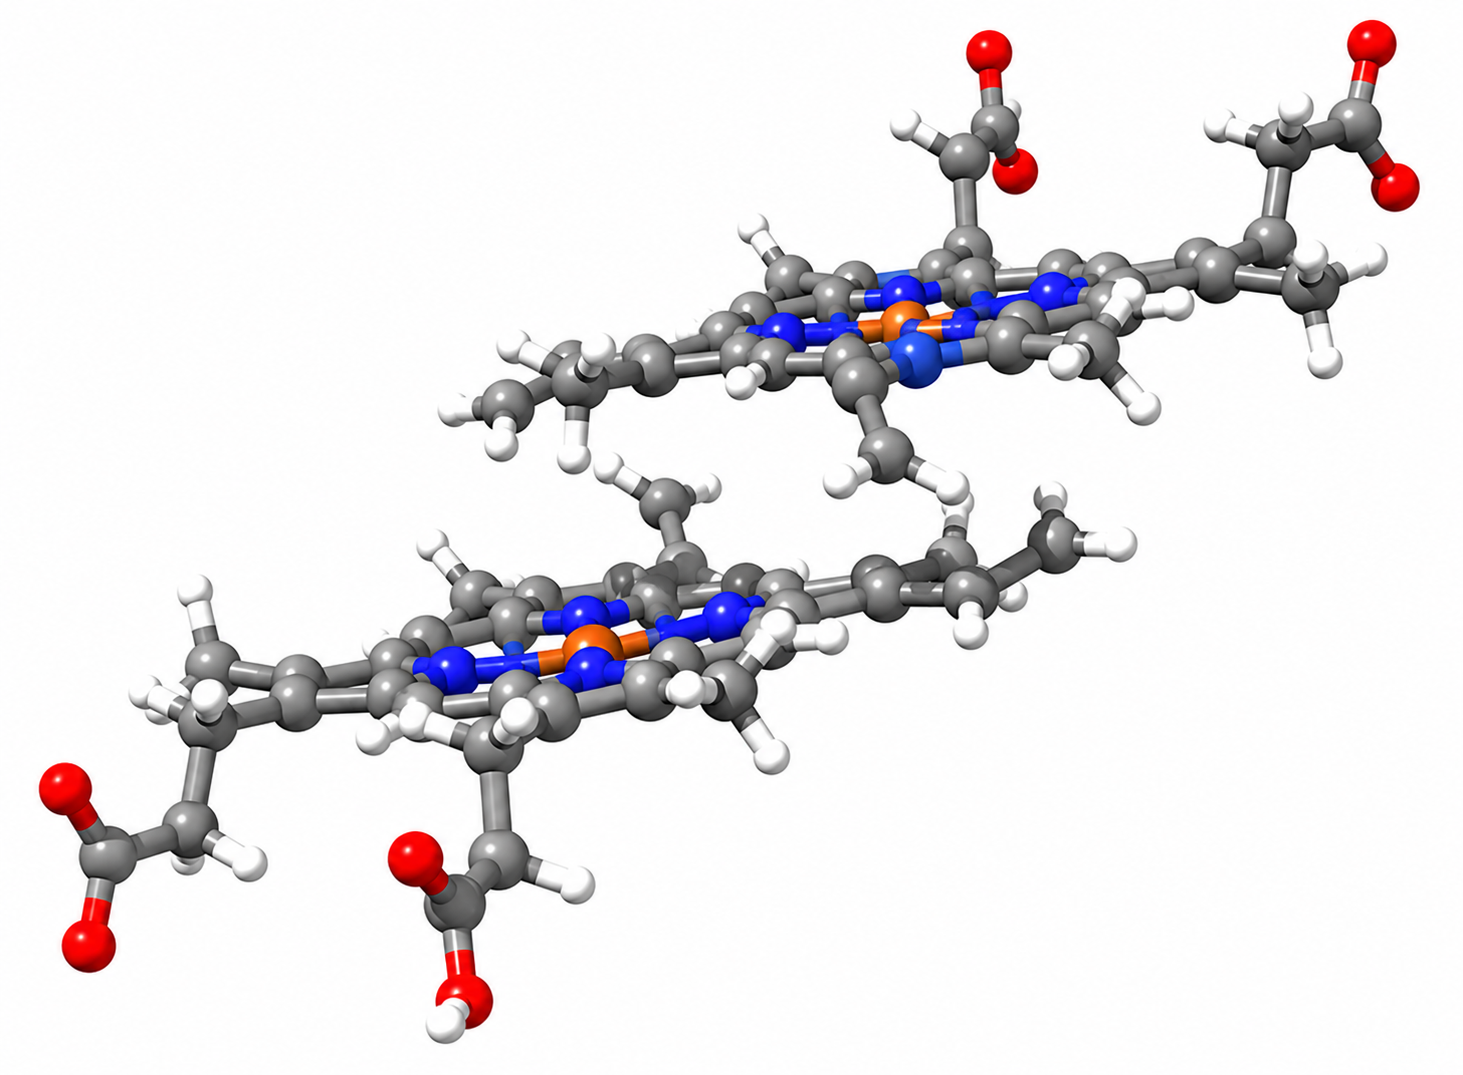
\includegraphics[height=0.55\textheight,keepaspectratio]{GU_pp.png}\\[0.5em]
      {\color{azul}\bfseries\small (b) Interacción $\pi$--$\pi$}\\[0.2em]
      {\footnotesize Más estable en medio acuoso
      {\scriptsize\color{gris}Klonis \emph{et al.} (2010); Ma \emph{et al.} (2025)}}
    \end{column}
  \end{columns}
\end{frame}

% =====================================================================
%  DIAPOSITIVA 2: Formación clásica multinivel
% =====================================================================
\begin{frame}{Formación clásica de los cristales de hemozoína}
  \begin{columns}[c,onlytextwidth]
    % Figura del ensamblaje
    \begin{column}{0.5\textwidth}
      \centering
      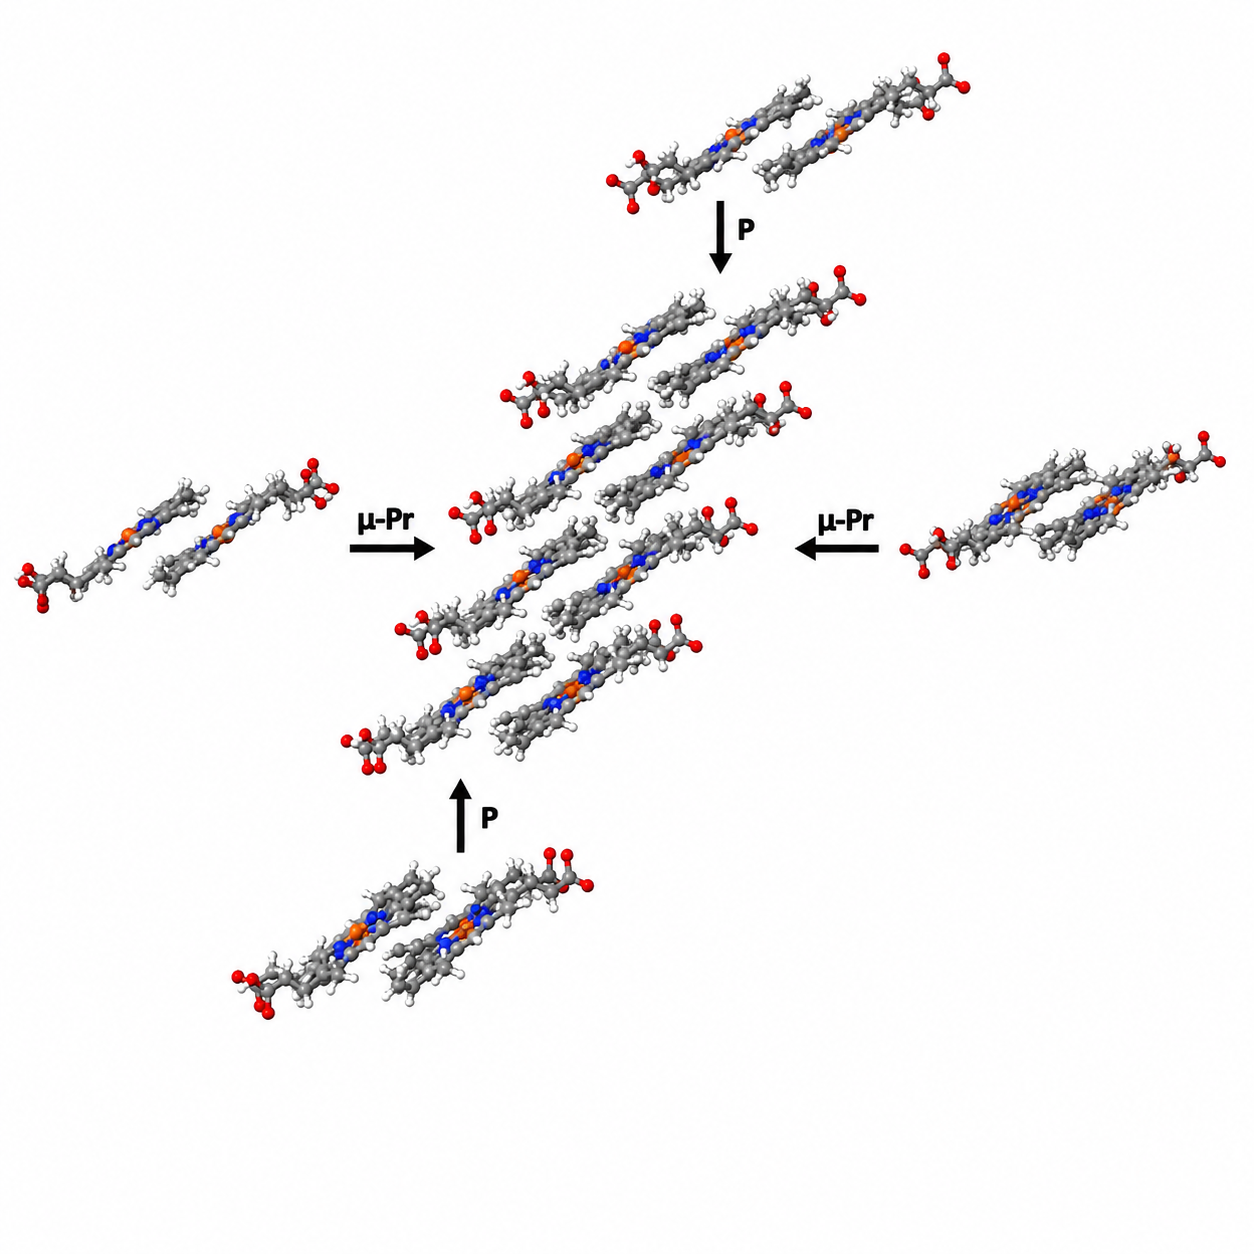
\includegraphics[width=\linewidth,height=0.70\textheight,keepaspectratio]{laywe.png}\\[0.4em]
      \fig{.}
    \end{column}

    % Explicación / Tabla por etapas
    \begin{column}{0.45\textwidth}
      \centering
      \small
      \renewcommand{\arraystretch}{1.25}
      \begin{tabular}{@{}l>{\raggedright\arraybackslash}p{0.52\linewidth}@{}}
        \toprule
        Etapa & Interacción determinante \\
        \midrule
        \textbf{Nucleación} & Formación de dímeros $\pi$--$\pi$ \\
        \textbf{1D (Columnas)} & Apilamiento direccional \textbf{tipo P} \\
        \textbf{2D (Láminas)}  & Enlaces de coordinación \textbf{$\mu$-Pr} \\
        \textbf{3D (Cristal)}  & van der Waals + \textbf{puentes de H} \\
        \bottomrule
      \end{tabular}

      \vspace{1.5cm}
      
    \end{column}
  \end{columns}
\end{frame}

% =====================================================================
%  DIAPOSITIVA 3: Interacciones moleculares (Ptype, mPr, HB)
% =====================================================================
\begin{frame}{Interacciones moleculares en la red cristalina}
  \framesubtitle{Modos de enlace específicos que controlan la cohesión direccional y la anisotropía.}
  \begin{columns}[T,onlytextwidth]
    % Interacción tipo P
    \begin{column}{0.32\textwidth}
      \centering
      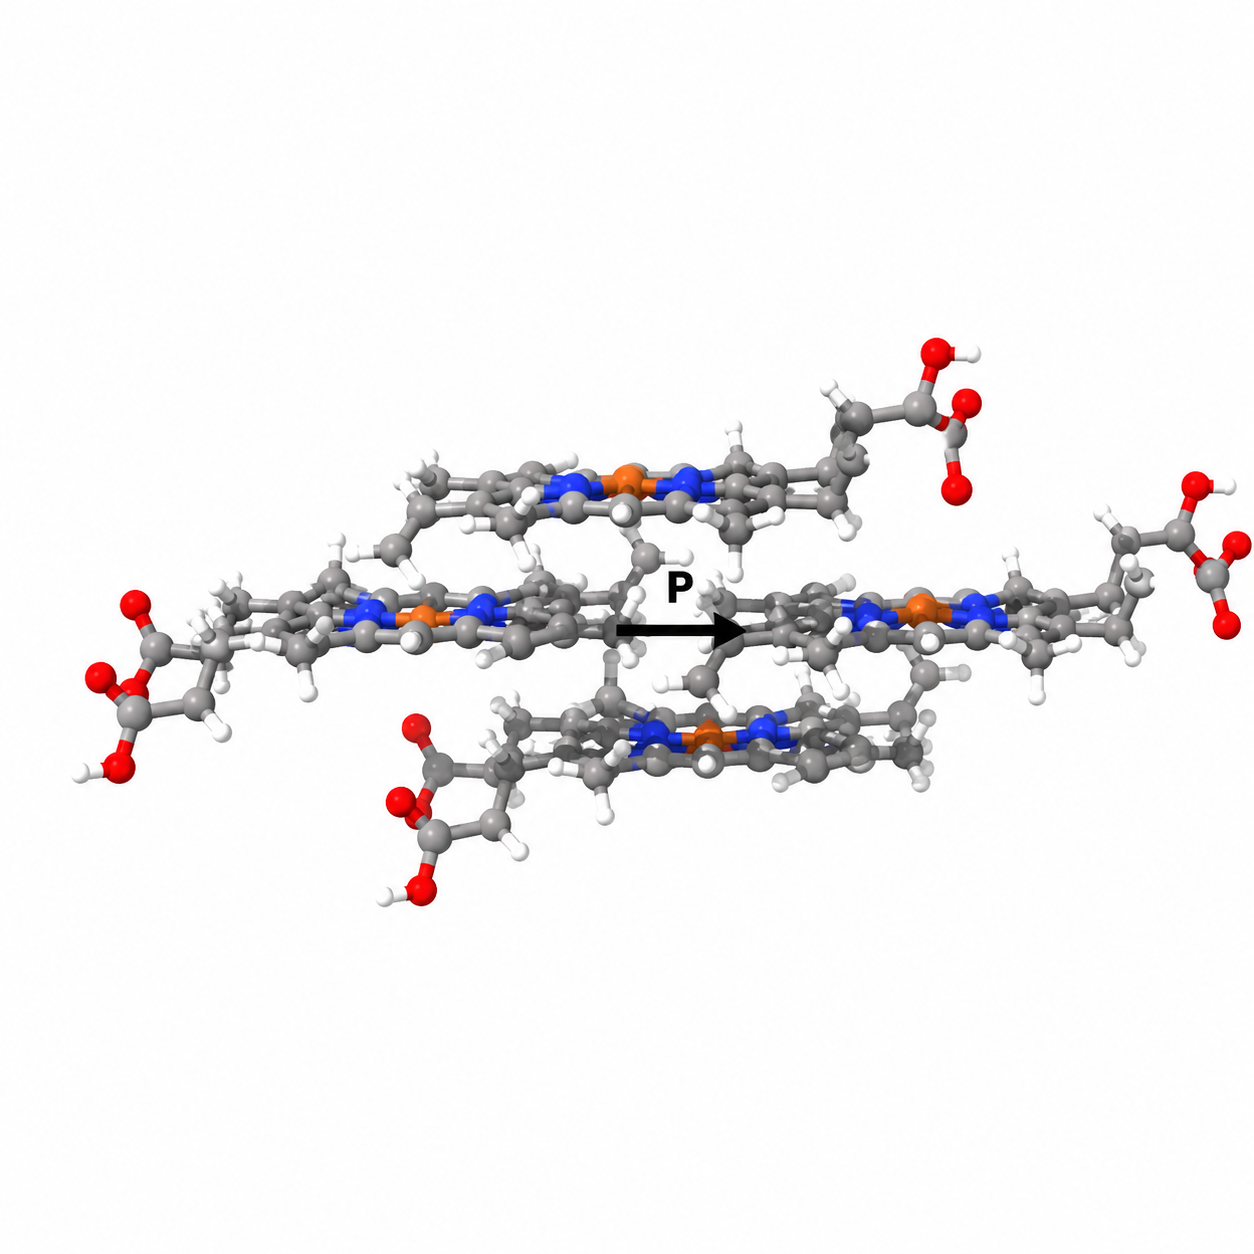
\includegraphics[width=0.95\linewidth,trim=0 60 0 60,clip]{Ptype.png}\\[0.5em]
      {\color{azul}\bfseries\small Interacción tipo P}\\[0.3em]
    \end{column}

    % Interacción mu-Pr
    \begin{column}{0.32\textwidth}
      \centering
      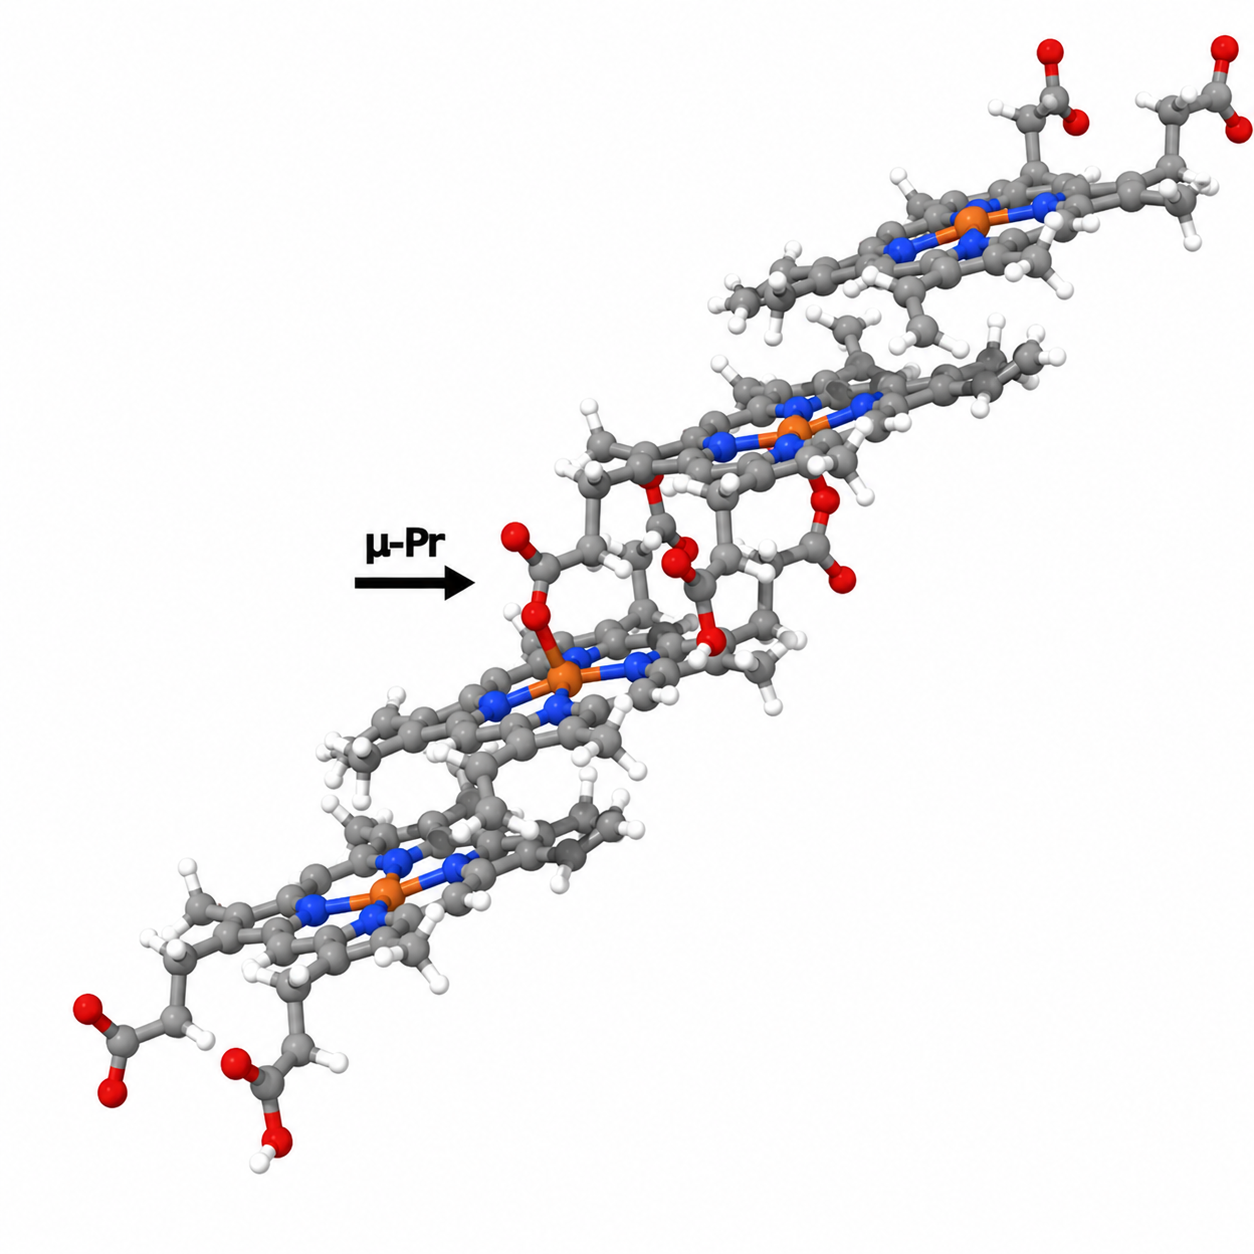
\includegraphics[width=0.95\linewidth,trim=0 60 0 60,clip]{mPr.png}\\[0.5em]
      {\color{azul}\bfseries\small Enlace $\mu$-Pr}\\[0.3em]
    \end{column}

    % Puentes de Hidrógeno
    \begin{column}{0.32\textwidth}
      \centering
      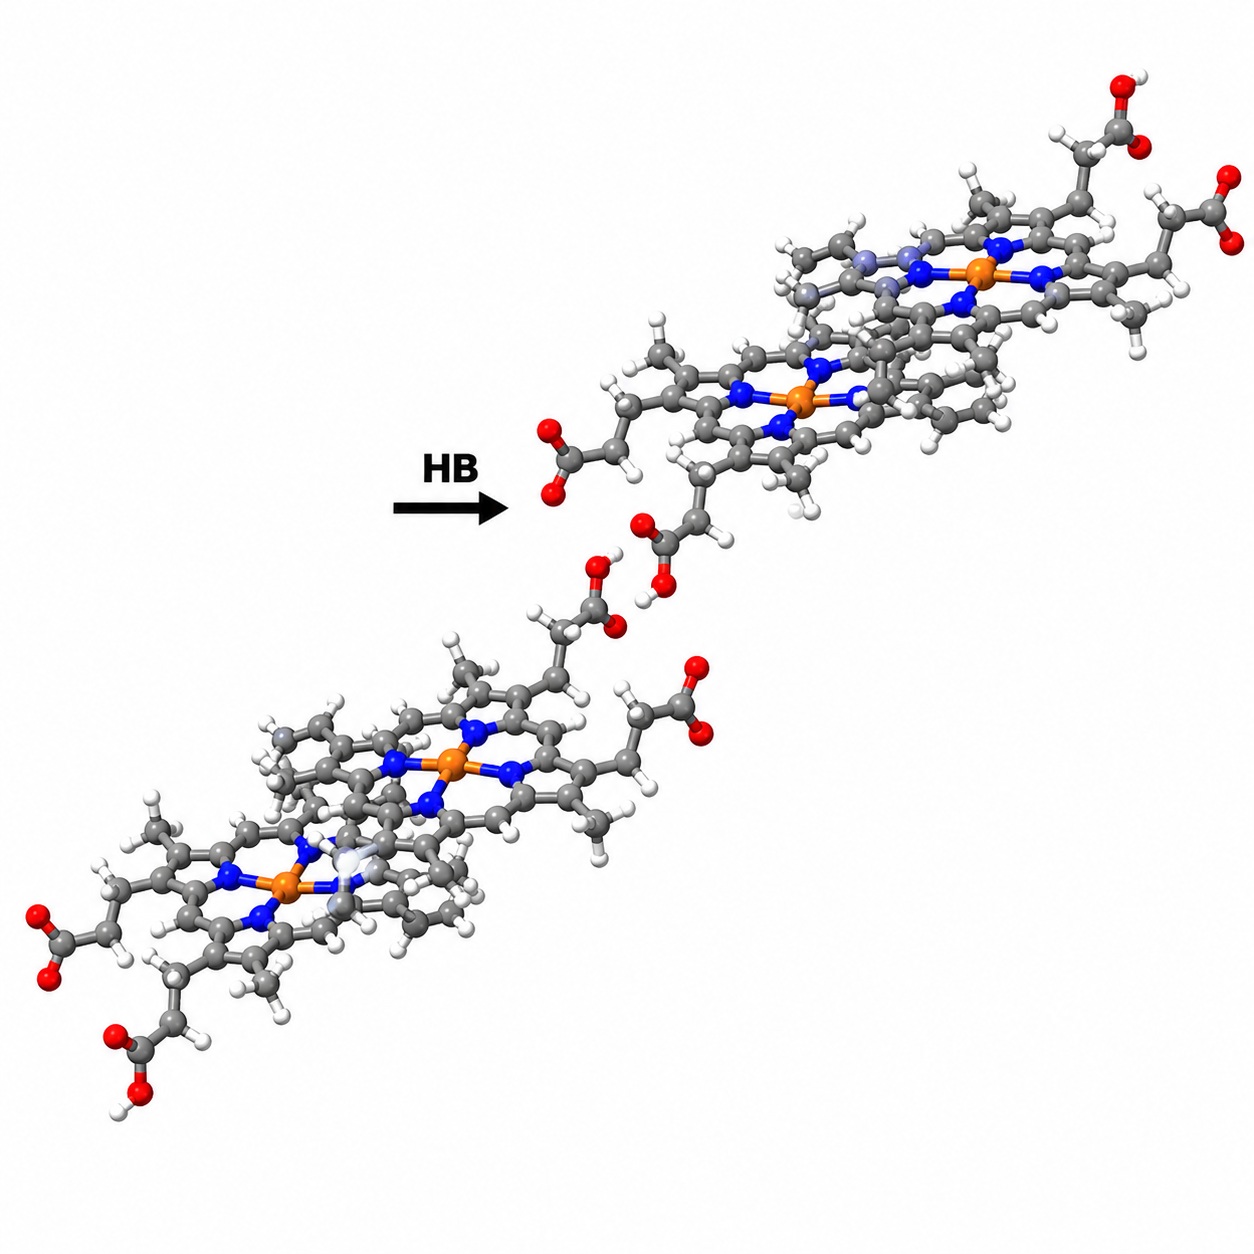
\includegraphics[width=0.95\linewidth,trim=0 60 0 60,clip]{HB.png}\\[0.5em]
      {\color{azul}\bfseries\small Puentes de H}\\[0.3em]
    \end{column}
  \end{columns}
\end{frame}

% ---------------------------------------------------------------- 5: MACE-POLAR
\begin{frame}{Escala atómica: potencial MACE-POLAR}
  \framesubtitle{MLIP: precisión cercana a DFT ($\mathcal{O}(N^3)$) con escalamiento lineal $\mathcal{O}(N)$.}
  \begin{columns}[c,onlytextwidth]
    \begin{column}{0.46\textwidth}
      \centering
      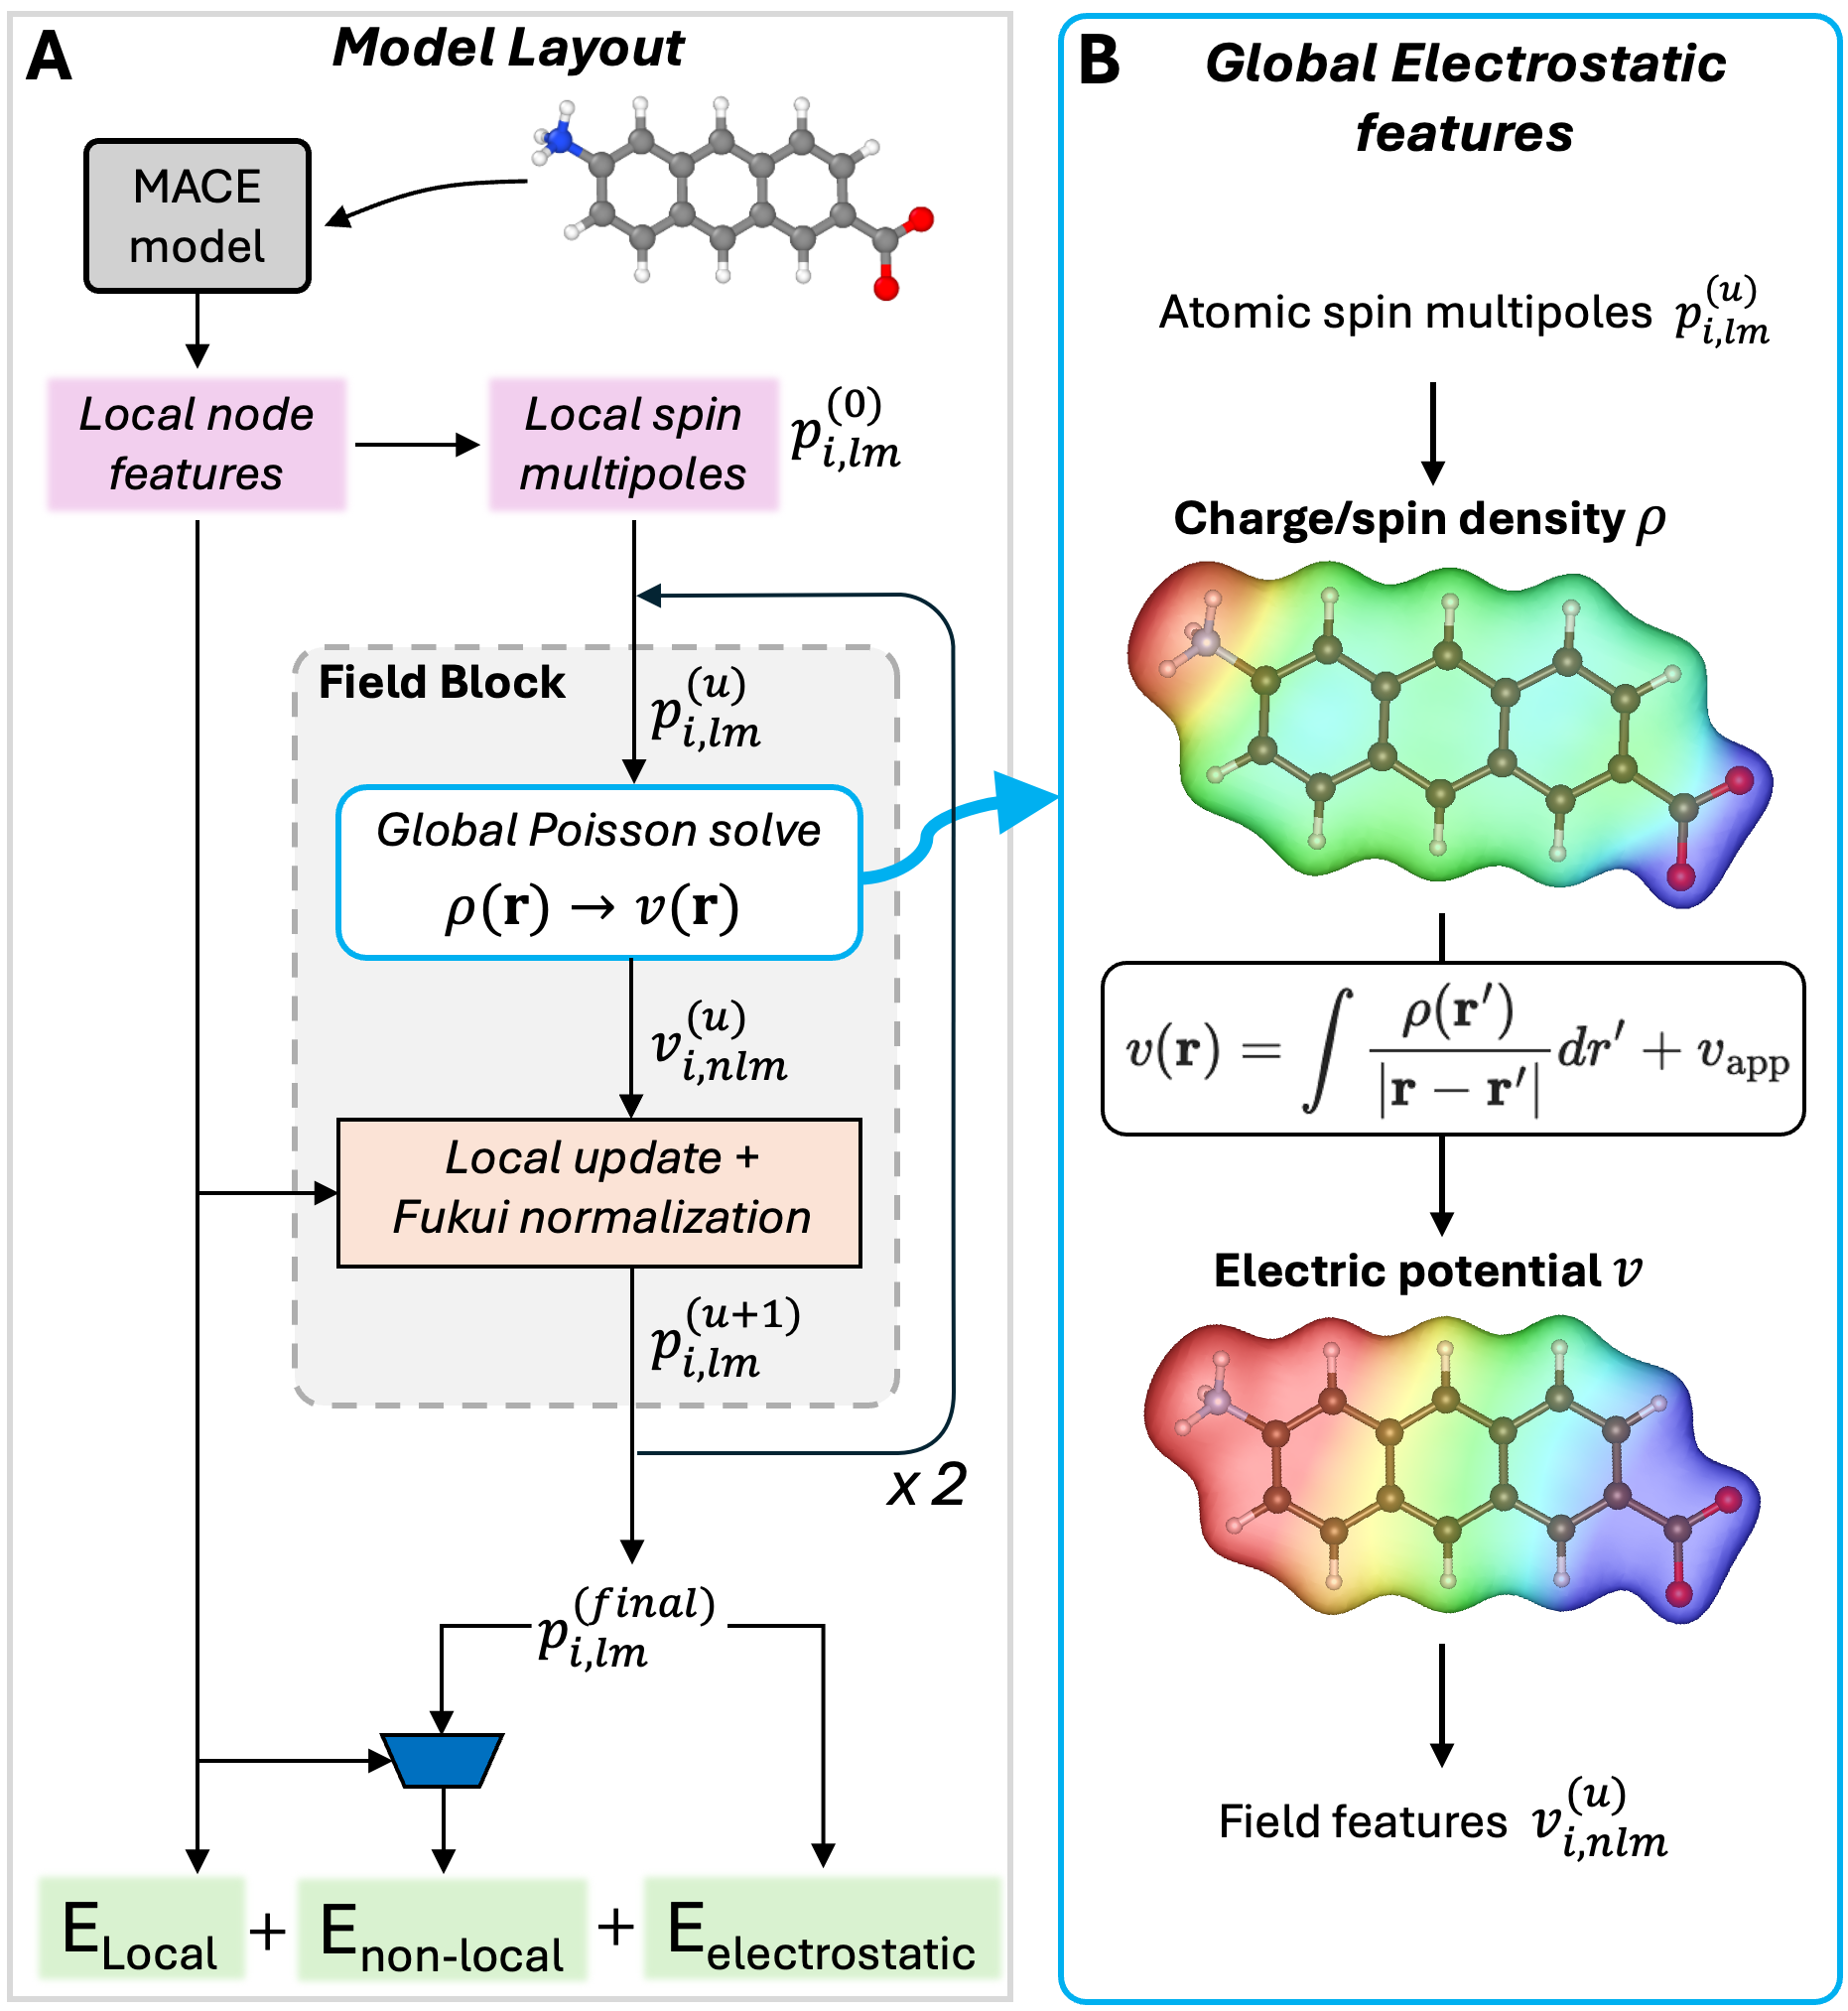
\includegraphics[height=0.55\textheight]{mace_polar_arq.png}\\
      \fig{Fig.~2. MACE-POLAR-1 (Batatia \emph{et al.}, 2026).}
    \end{column}
    \begin{column}{0.51\textwidth}
      \small
      \begin{itemize}\setlength{\itemsep}{0.6em}
        \item \textbf{MACE}: red neuronal de paso de mensajes \textbf{equivariante} (armónicos esféricos, muchos cuerpos) $\Rightarrow E_{\text{local}}$
        \item \textbf{POLAR}: multipolos de espín-carga $\to$ Poisson global $\rho(\mathbf r)\to v(\mathbf r)$ $\Rightarrow E_{\text{elec}} + E_{\text{no-local}}$
        \item Entrenado en \textbf{OMol25} ($\omega$B97M-V): electrostática de largo alcance
        \item UC $\pi$--$\pi$: \textbf{148 átomos}; relajación de celda y posiciones con ASE (L-BFGS)
      \end{itemize}
    \end{column}
  \end{columns}
\end{frame}

% ---------------------------------------------------------------- 6: Energías Epb
\begin{frame}{Energías de enlace $E_{pb}$ por dirección}
  \begin{columns}[c,onlytextwidth]
    \begin{column}{0.50\textwidth}
      \centering
      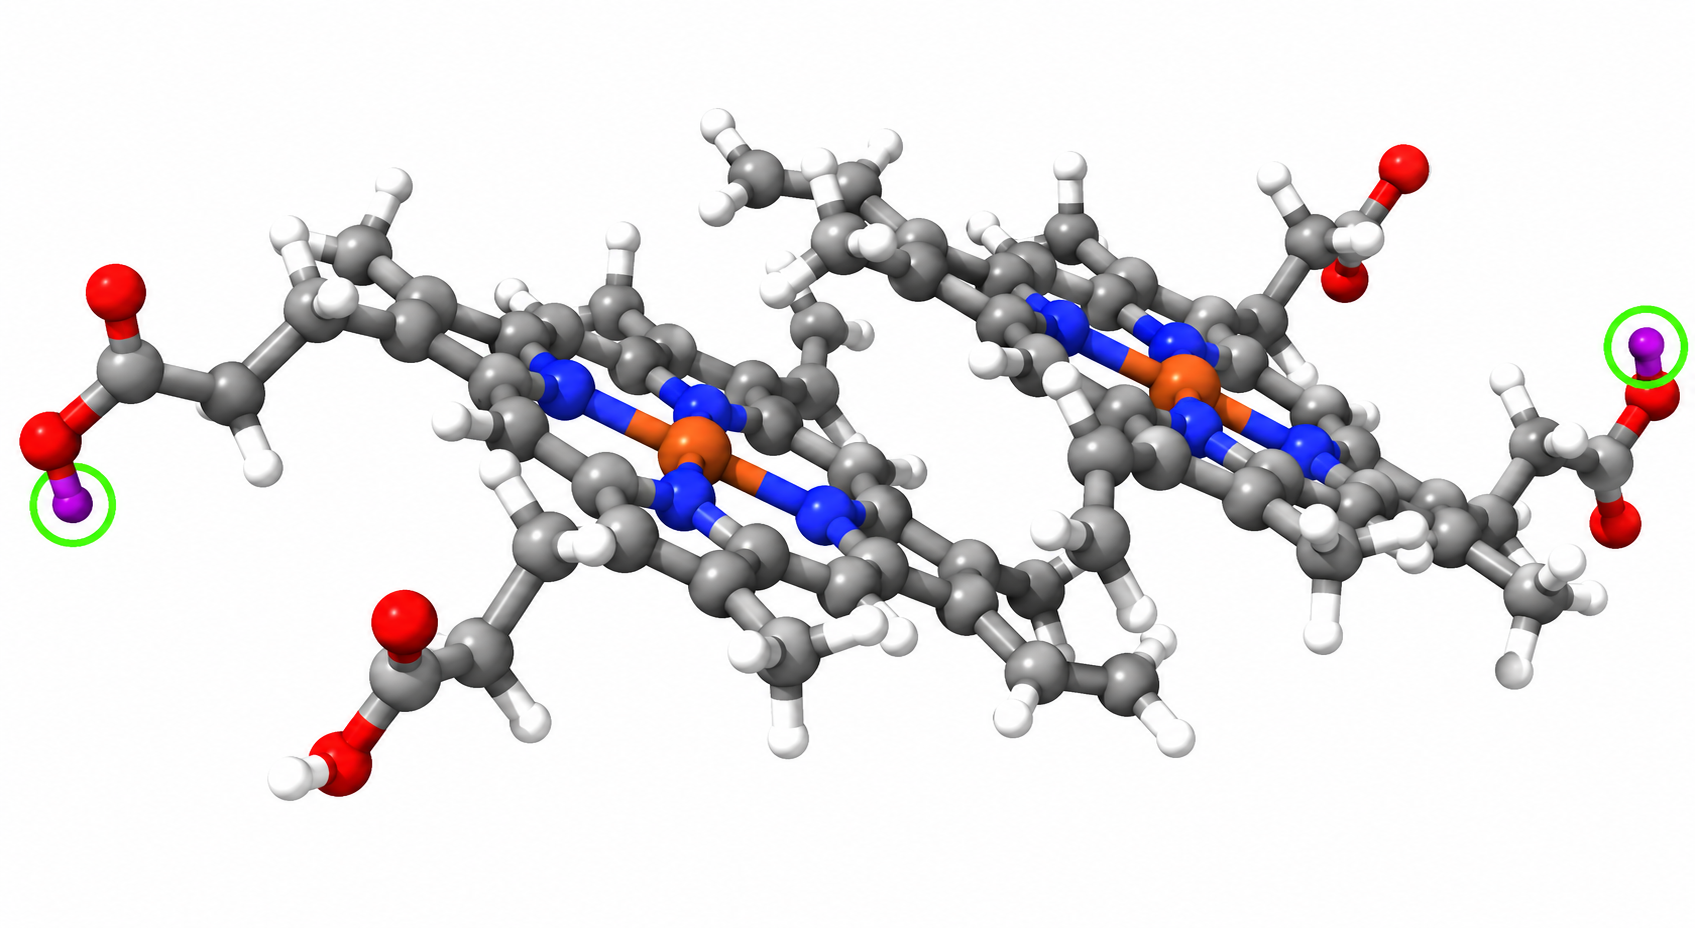
\includegraphics[width=\linewidth,height=0.40\textheight,keepaspectratio]{H_extra_c.png}\\
      \fig{Fig.~3. Oxígenos externos saturados con H: evita el colapso de los carboxilos en vacío.}\\[0.4em]
      \small
      \begin{align}
        E_{\mu\text{-Pr}} &= E_{\text{dim}} + E_{\text{H}_2} - 2E_{\text{UC}} \tag{1}\\
        E_{pb} &= E_{\text{dim}} - 2E_{\text{UC}} \tag{2}
      \end{align}
    \end{column}
    \begin{column}{0.47\textwidth}
      \centering\small
      \renewcommand{\arraystretch}{1.2}
      \begin{tabular}{@{}lc@{}}
        \toprule
        Dirección & $E_{pb}$ (eV) \\
        \midrule
        $\mu$-propionato      & $-0.7609$ \\
        Puente de H           & $-0.7420$ \\
        P--P                  & $\mathbf{-2.1994}$ \\
        \midrule
        Promedio total        & $-1.2341$ \\
        \bottomrule
      \end{tabular}\\[0.6em]
      \begin{block}{\centering Entrada del kMC anisotrópico}
        \centering
        $E_{pb_x}\leftarrow\mu$-Pr \qquad $E_{pb_y}\leftarrow$ P--P
      \end{block}
      {\footnotesize Relajación en vacío en dos etapas (L-BFGS): solo H añadidos $\to$ todos los átomos}
    \end{column}
  \end{columns}
\end{frame}

% ---------------------------------------------------------------- 7: Cinética
\begin{frame}{Cinética de cristalización: de la CNT a dos etapas}
  \framesubtitle{Curvas de conversión sigmoidales: inducción lenta, crecimiento acelerado y saturación.}
  \begin{columns}[c,onlytextwidth]
    \begin{column}{0.41\textwidth}
      \centering
      {\color{azul}\bfseries\small Teoría clásica de nucleación}\\[0.2em]
      \begin{tikzpicture}[x=1.45cm,y=0.9cm,>=stealth]
        \draw[->,gris] (0,0) -- (1.85,0) node[right,font=\scriptsize]{$r$};
        \draw[->,gris] (0,-1.05) -- (0,1.3) node[above,font=\scriptsize]{$\Delta G$};
        \draw[dashed,azul!60,domain=0:0.93,samples=30] plot (\x,{1.5*\x*\x});
        \draw[dashed,acento!60,domain=0:1.0,samples=30] plot (\x,{-\x*\x*\x});
        \draw[very thick,azul,domain=0:1.72,samples=50] plot (\x,{1.5*\x*\x-\x*\x*\x});
        \draw[dotted,gris] (1,0) -- (1,0.5);
        \fill[acento] (1,0.5) circle (0.05);
        \node[font=\scriptsize,below] at (1,0) {$r^{*}$};
        \node[font=\tiny,azul!70,anchor=west] at (0.62,1.15) {$4\pi r^2\gamma$};
        \node[font=\tiny,acento!80,anchor=west] at (0.55,-0.75) {$-\tfrac43\pi r^3\Delta G_V$};
      \end{tikzpicture}
      \small
      \begin{align}
        \Delta G(r) &= -\tfrac{4}{3}\pi r^{3}\Delta G_V + 4\pi r^{2}\gamma \tag{3}\\
        r^{*} &= \frac{2\gamma}{\Delta G_V} \tag{4}
      \end{align}
    \end{column}
    \begin{column}{0.56\textwidth}
      \small
      {\color{azul}\bfseries Avrami}\ {\footnotesize (supone la UC ya formada)}
      \begin{equation}
        X(t) = X_0\left[1-\exp\!\left(-kt^{n}\right)\right],\quad n=n_d+n_N \tag{5}
      \end{equation}
      {\color{azul}\bfseries Pasternack}\ {\footnotesize (fenomenológico, bifásico)}
      \begin{equation}
        X(t) = y_0 - y_1 e^{-kt^{n}} - y_2 e^{-k_s t} \tag{6}
      \end{equation}
      \vspace{-0.6em}
      \begin{block}{Dos etapas (Parra, 2023)}
        \vspace{-0.4em}
        \begin{equation}
          X(t) = \alpha - \frac{\alpha}{\alpha k_1 t + 1} + \frac{\beta}{1+\exp\!\left(-\beta k_2 t + D\right)} \tag{7}
        \end{equation}
      \end{block}
    \end{column}
  \end{columns}
\end{frame}

% ---------------------------------------------------------------- 8: Nucleación 2D
\begin{frame}{Nucleación 2D y regímenes de crecimiento superficial}
  \framesubtitle{La sobresaturación $\sigma$ controla el mecanismo de crecimiento de la cara cristalina.}
  \begin{columns}[c,onlytextwidth]
    \begin{column}{0.46\textwidth}
      \centering
      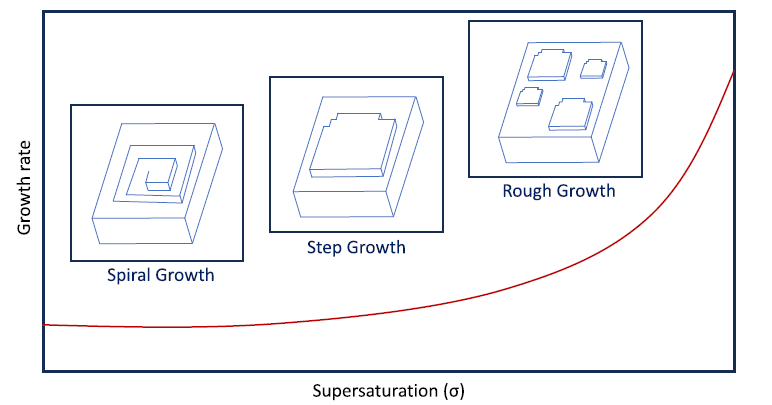
\includegraphics[width=0.62\linewidth]{growth_regimes.png}\\
      \fig{Fig.~4. Regímenes de crecimiento según la sobresaturación $\sigma$.}\\[0.3em]
      \footnotesize
      \renewcommand{\arraystretch}{1.15}\setlength{\tabcolsep}{4pt}
      \begin{tabular}{@{}lll@{}}
        \toprule
        $\sigma$ & Régimen & Mecanismo \\
        \midrule
        baja  & espiral & dislocaciones, sitios \textit{kink} \\
        media & escalón & nucleación 2D de islas \\
        alta  & rugoso  & adátomos aislados \\
        \bottomrule
      \end{tabular}
    \end{column}
    \begin{column}{0.52\textwidth}
      \setlength{\abovedisplayskip}{2pt}\setlength{\belowdisplayskip}{2pt}
      {\color{azul}Fuerza impulsora}
      \begin{equation}
        \Delta\mu = \kB T\ln\frac{C}{C_{eq}} = \kB T\ln(\sigma+1) \tag{8}
      \end{equation}
      {\footnotesize $C$: concentración de UC;\ $C_{eq}$: saturación;\ $\sigma = C/C_{eq}-1$}\\[0.1em]
      {\color{azul}Creación de una nueva interfaz plana}
      \begin{equation}
        \Delta G = -N\Delta\mu + \gamma_{edge}A \tag{9}
      \end{equation}
      {\footnotesize $-N\Delta\mu$: favorece el cristal \quad $\gamma_{edge}A$: barrera superficial}\\[0.1em]
      \begin{block}{}
        \centering\footnotesize
        $\sigma\uparrow\ \Rightarrow\ \Delta\mu\uparrow$:\ espiral $\to$ escalón (nucleación 2D) $\to$ rugoso
      \end{block}
    \end{column}
  \end{columns}
\end{frame}

% ---------------------------------------------------------------- 9: kMC y BKL
\begin{frame}{Monte Carlo cinético (kMC) y algoritmo BKL}
  \framesubtitle{\textbf{kMC:} evolución estocástica por eventos discretos con probabilidades físicas y \textbf{tiempo real}.}
  \begin{columns}[c,onlytextwidth]
    \begin{column}{0.47\textwidth}
      \centering
      \begin{tikzpicture}[x=0.78cm,y=0.46cm,>=stealth]
        \draw[thick,azul] plot[smooth,tension=0.7] coordinates
          {(0,2.1) (0.8,0.45) (1.6,1.75) (2.6,0.8) (3.5,1.95) (4.4,0.3) (5.3,1.9) (5.8,2.2)};
        \node[font=\scriptsize,gris] at (0.8,0.1) {$i$};
        \node[font=\scriptsize,gris] at (2.6,0.45) {$j$};
        \fill[acento] (0.8,0.62) circle (0.11);
        \draw[gris] (0.45,0.95) -- (0.6,0.8) -- (0.72,0.98) -- (0.86,0.8) -- (1.0,0.98) -- (1.15,0.82);
        \draw[<->,gris] (1.6,0.45) -- node[right,font=\scriptsize]{$\Delta E_{ij}$} (1.6,1.72);
        \draw[dashed,gris] (0.8,0.45) -- (1.6,0.45);
        \draw[->,thick,acento] (0.95,0.75) .. controls (1.2,2.6) and (2.2,2.4) .. node[pos=0.5,above,font=\scriptsize,acento]{$k_{ij}$} (2.45,1.0);
        \draw[->,thick,acento!70] (2.75,1.0) to[out=70,in=110] (4.25,0.55);
        \node[font=\scriptsize] at (2.9,-0.55) {coordenada de configuración};
        \node[font=\scriptsize,rotate=90] at (-0.35,1.1) {energía};
      \end{tikzpicture}
      \small
      \setlength{\abovedisplayskip}{2pt}\setlength{\belowdisplayskip}{2pt}
      \begin{align}
        \frac{dP_i}{dt} &= \sum_{j\neq i}\left[k_{ji}P_j - k_{ij}P_i\right] \tag{10}\\
        k_{ij} &= \nu_{ij}\exp\!\left(-\frac{\Delta E_{ij}}{\kB T}\right) \tag{11}
      \end{align}
    \end{column}
    \begin{column}{0.50\textwidth}
      {\color{azul}\bfseries Algoritmo BKL (Gillespie)}
      \small
      \setlength{\abovedisplayskip}{2pt}\setlength{\belowdisplayskip}{2pt}
      \begin{align}
        k_{tot} &= \sum_{j\neq i} k_{ij} \tag{12}\\[0.2em]
        \sum_{l<j} k_{il} &< r_1\,k_{tot} \le \sum_{l\le j} k_{il} \tag{13}
      \end{align}
      \vspace{-0.4em}
      \begin{block}{}
        \vspace{-0.3em}
        \begin{equation}
          \Delta t = -\frac{\ln r_2}{k_{tot}}, \qquad r_2\in(0,1] \tag{14}
        \end{equation}
      \end{block}
      {\footnotesize Ejecutar evento, actualizar tasas y avanzar tiempo\\
      Intervalos de Poisson: $\Delta t \propto 1/k_{tot}$}
    \end{column}
  \end{columns}
\end{frame}

% ---------------------------------------------------------------- 10: Modelo SOS
\begin{frame}{Modelo kMC 3D: red SOS y sitios de adsorción}
  \framesubtitle{Adaptación de Nagpal \emph{et al.} (2024) $+$ \textbf{anisotropía} $+$ evento de \textbf{incorporación}.}
  \begin{columns}[c,onlytextwidth]
    \begin{column}{0.44\textwidth}
      \centering
      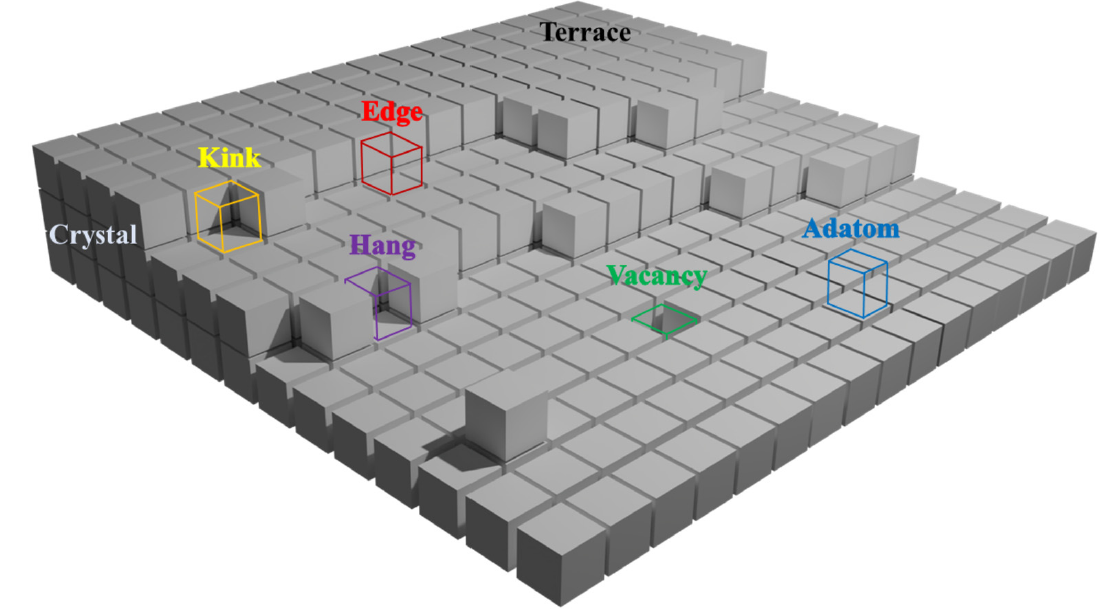
\includegraphics[width=0.85\linewidth]{general_model.png}\\
      \fig{Fig.~5. Sitios de adsorción del modelo SOS.}\\[0.3em]
      \scriptsize
      \renewcommand{\arraystretch}{1.15}
      \setlength{\tabcolsep}{2.5pt}
      \begin{tabular}{@{}lccccc@{}}
        \toprule
        Sitio & adátomo & borde & \textit{kink} & colgante & vacante \\
        \midrule
        $n$   & 0 & 1 & 2 & 3 & 4 \\
        \bottomrule
      \end{tabular}\\[0.3em]
      {\scriptsize\color{gris}SOS: sin vacantes internas ni voladizos}
    \end{column}
    \begin{column}{0.54\textwidth}
      \small
      \setlength{\abovedisplayskip}{2pt}\setlength{\belowdisplayskip}{2pt}
      \begin{itemize}\setlength{\itemsep}{0.2em}
        \item Red $80\times80$, fronteras periódicas, vecindad de von Neumann
        \item \textit{Solid-on-solid}: cada sitio guarda una \textbf{altura}
      \end{itemize}
      \begin{block}{Energía libre por UC adsorbida}
        \vspace{-0.5em}
        \begin{equation}
          \Delta G_{UC} = -\Delta\mu + \gamma_{edge}\,n\,A_f \tag{15}
        \end{equation}
      \end{block}
      {\footnotesize $n$ vecinos $\Rightarrow$ la adsorción \textbf{distingue} el tipo de sitio}\\[0.1em]
      {\footnotesize Eventos: \textbf{adsorción} · \textbf{desorción} · \textbf{migración} · \textbf{incorporación}}
    \end{column}
  \end{columns}
\end{frame}

% ---------------------------------------------------------------- 11: Tasas de transición
\begin{frame}{Modelo kMC 3D: tasas de transición}
  \framesubtitle{\textbf{Anisotropía:} $E_{pb_x}\neq E_{pb_y}$; con $E_{pb_x}=E_{pb_y}$ se recupera el modelo isotrópico.}
  \begin{columns}[c,onlytextwidth]
    \begin{column}{0.73\textwidth}
      \footnotesize
      \setlength{\abovedisplayskip}{0pt}\setlength{\belowdisplayskip}{0pt}\setlength{\jot}{0pt}
      \begin{align}
        k_{a_n} &= K_0^{+}\exp\!\left(\frac{\Delta\mu}{\kB T} + n_x\frac{\delta_x}{\Delta\mu} + n_y\frac{\delta_y}{\Delta\mu}\right) \tag{16}\\
        k_{d_n} &= K_0^{+}\exp\!\left(\frac{\phi}{\kB T} - n_x\frac{E_{pb_x}}{\kB T} - n_y\frac{E_{pb_y}}{\kB T}\right) \tag{17}\\
        k_{m_n} &= K_0^{+}\exp\!\left(\frac{\phi}{\kB T} + \frac{E_{pb_x}+E_{pb_y}}{2\kB T} - n_x\frac{E_{pb_x}}{\kB T} - n_y\frac{E_{pb_y}}{\kB T}\right) \tag{18}\\
        k_{i_n} &= K_{inc}^{+}\exp\!\left(n_x\frac{E_{pb_x}}{\kB T} + n_y\frac{E_{pb_y}}{\kB T}\right) \tag{19}
      \end{align}
      {\footnotesize $\phi$: enlace por UC en la red llena;\ $E_{pb}$: energía por enlace;\ $n_x,n_y\in\{0,1,2\}$\\
       $\Delta\mu$ baja $\Rightarrow$ dominan sitios con más vecinos;\ $\Delta\mu$ alta $\Rightarrow$ adsorción rápida\\
       Tasa total $W_{tot}=\sum_{j\in\{a,d,m,i\}}\sum_n M_n\,k_{j_n}$;\ evento $j$ con $P_j = W_j/W_{tot}$}
    \end{column}
    \begin{column}{0.25\textwidth}
      \centering
      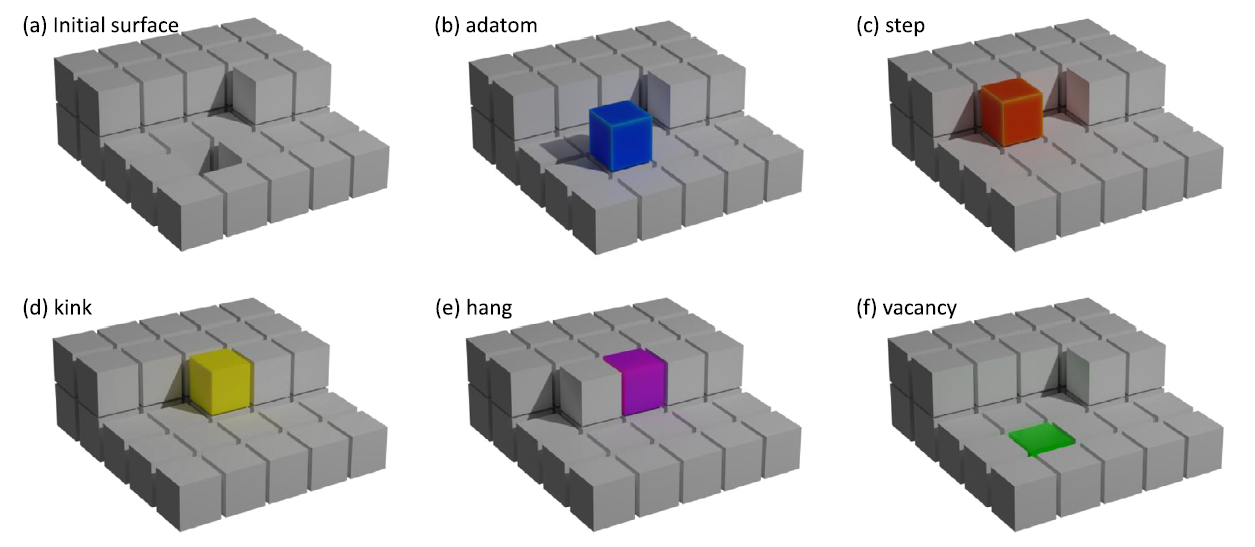
\includegraphics[width=\linewidth]{adsortion.png}\\
      \fig{Fig.~6. Adsorción en sitios.}\\[0.3em]
      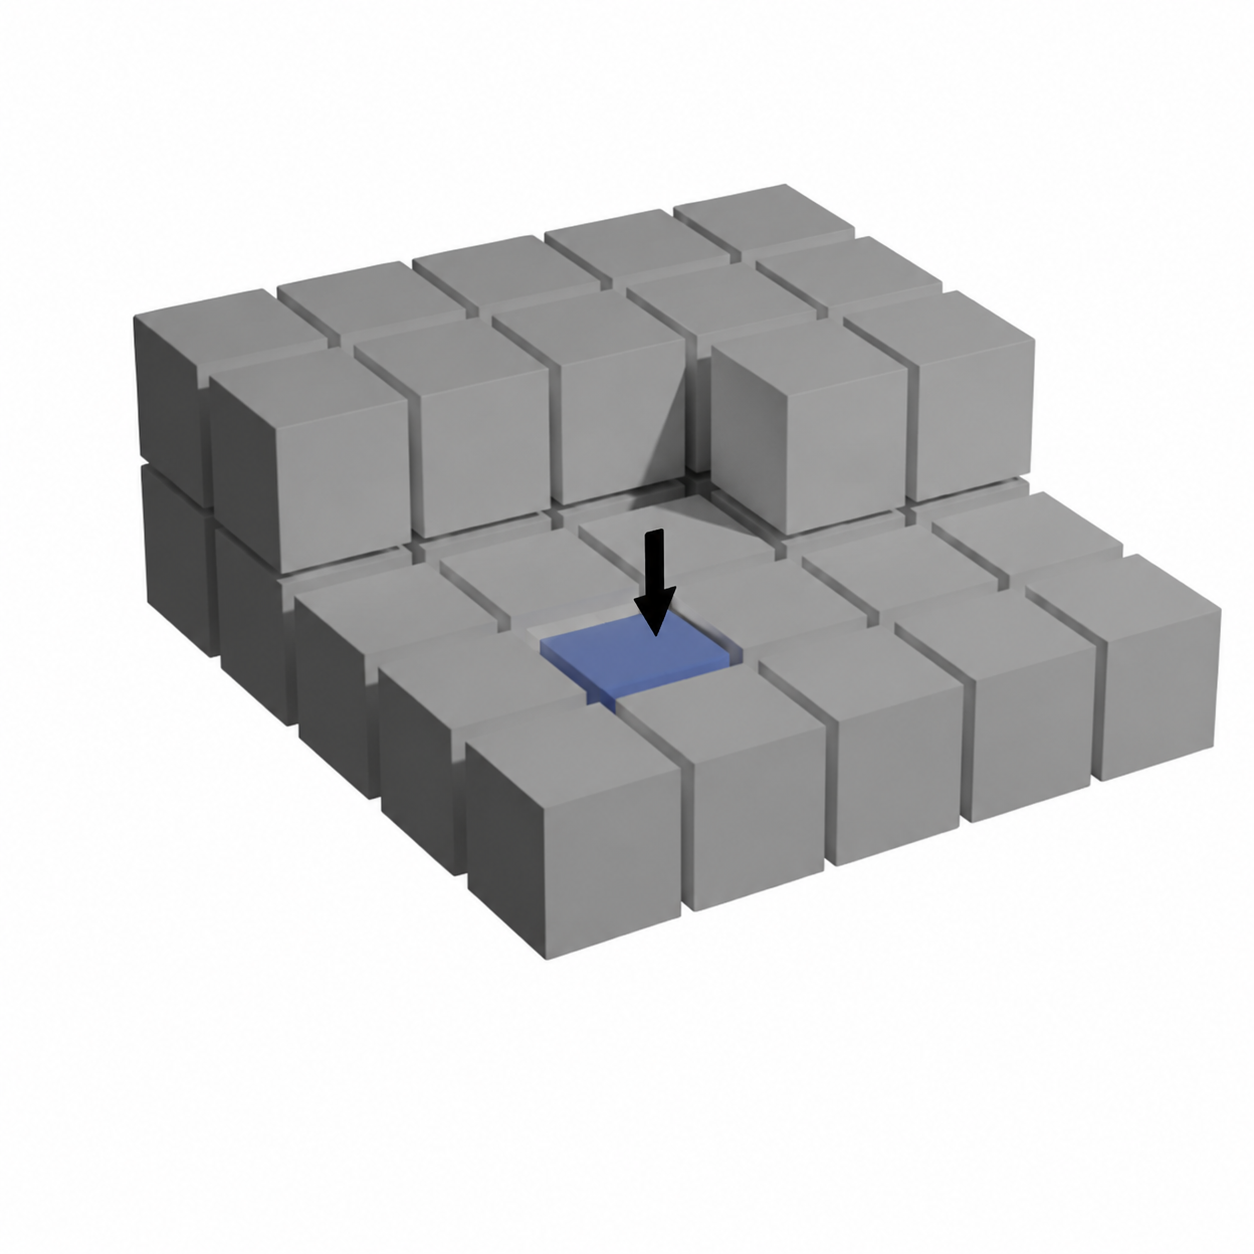
\includegraphics[width=0.48\linewidth]{incorporation.png}\\
      \fig{Fig.~7. Incorporación: nueva.}
    \end{column}
  \end{columns}
\end{frame}

% ---------------------------------------------------------------- 12: Cinética de conversión
\begin{frame}{Resultados: cinética de conversión a $\beta$-hematina}
  \begin{columns}[c,onlytextwidth]
    \begin{column}{0.60\textwidth}
      \centering
      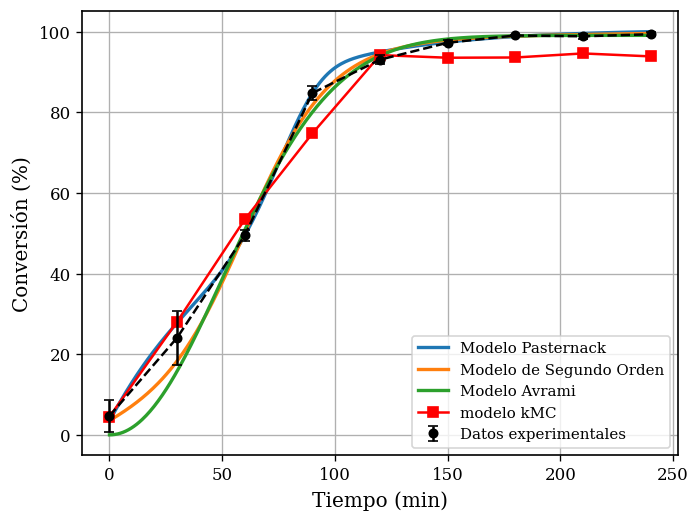
\includegraphics[height=0.60\textheight]{3d_conv.png}
    \end{column}
    \begin{column}{0.36\textwidth}
      \small
      \renewcommand{\arraystretch}{1.2}\setlength{\tabcolsep}{3pt}
      \begin{tabular}{@{}lcc@{}}
        \toprule
        Modelo & $R^2$ & RMSE \\
        \midrule
        Pasternack   & 0.998 & 1.49 \\
        2.º orden    & 0.995 & 2.28 \\
        Avrami       & 0.989 & 3.60 \\
        \midrule
        \textbf{kMC 3D} & \textbf{0.971} & \textbf{4.69} \\
        \bottomrule
      \end{tabular}\\[0.5em]
      Red $80\times80$\\
      $t\in[0,240]$ min
    \end{column}
  \end{columns}
  \vspace{0.3em}
  \fig{Fig.~8. Conversión (\%) vs.\ tiempo: kMC, modelos cinéticos (ecs.~5--7) y datos experimentales.}
\end{frame}

% ---------------------------------------------------------------- 13: Morfología kMC
\begin{frame}{Resultados: morfología superficial (kMC 3D anisotrópico)}
  \begin{columns}[c,onlytextwidth]
    \begin{column}{0.63\textwidth}
      \centering
      \setlength{\tabcolsep}{1pt}
      \renewcommand{\arraystretch}{0.8}
      \begin{tabular}{@{}r@{\hspace{4pt}}ccc@{}}
        & {\scriptsize $t=30$ min} & {\scriptsize $t=60$ min} & {\scriptsize $t=240$ min} \\
        {\scriptsize $\sigma=0.38$} & \snap{0.165\textheight}{aniso_c_1.png} & \snap{0.165\textheight}{aniso_c_2.png} & \snap{0.165\textheight}{aniso_c_3.png} \\
        {\scriptsize $\sigma=1.5$}  & \snap{0.165\textheight}{aniso_d_2.png} & \snap{0.165\textheight}{aniso_d_1.png} & \snap{0.165\textheight}{aniso_d_3.png} \\
        {\scriptsize $\sigma=2.7$}  & \snap{0.165\textheight}{aniso_e_1.png} & \snap{0.165\textheight}{aniso_e_2.png} & \snap{0.165\textheight}{aniso_e_3.png}
      \end{tabular}\\[0.1em]
      \fig{Fig.~9. Snapshots del modelo 3D anisotrópico (red $80\times80$).}
    \end{column}
    \begin{column}{0.35\textwidth}
      \centering
      {\color{azul}\bfseries\scriptsize Parámetros}\\[0.1em]
      \scriptsize
      \renewcommand{\arraystretch}{0.92}\setlength{\tabcolsep}{3pt}
      \begin{tabular}{@{}lr@{}}
        \toprule
        \multicolumn{2}{@{}l}{\textbf{MACE}} \\
        $E_{pb_x}$ ($\mu$-Pr) & $-0.7609$\,eV \\
        $E_{pb_y}$ (P--P)     & $-2.1994$\,eV \\
        \midrule
        \multicolumn{2}{@{}l}{\textbf{Optimización bayesiana}} \\
        $\phi/\kB T$  & 1.48 \\
        $\delta$      & 1.78 \\
        $K_0^{+}$     & 11.67 \\
        $K_{inc}^{+}$ & 0.507 \\
        \bottomrule
      \end{tabular}\\[0.2em]
      \begin{block}{\centering Lectura}
        \centering\footnotesize
        $\sigma\uparrow$ $\Rightarrow$ más núcleos, islas menos definidas $\Rightarrow$ \textbf{mayor rugosidad}
      \end{block}
      {\scriptsize\color{gris}Misma tendencia en el modelo isotrópico.}
    \end{column}
  \end{columns}
\end{frame}

% ---------------------------------------------------------------- 14: Comparación AFM
\begin{frame}{Comparación con experimento: AFM de $\beta$-hematina}
  \framesubtitle{Olafson \emph{et al.} (2017), cara (100): de nucleación 2D y escalones a una interfaz rugosa.}
  \begin{columns}[c,onlytextwidth]
    \begin{column}{0.50\textwidth}
      \centering
      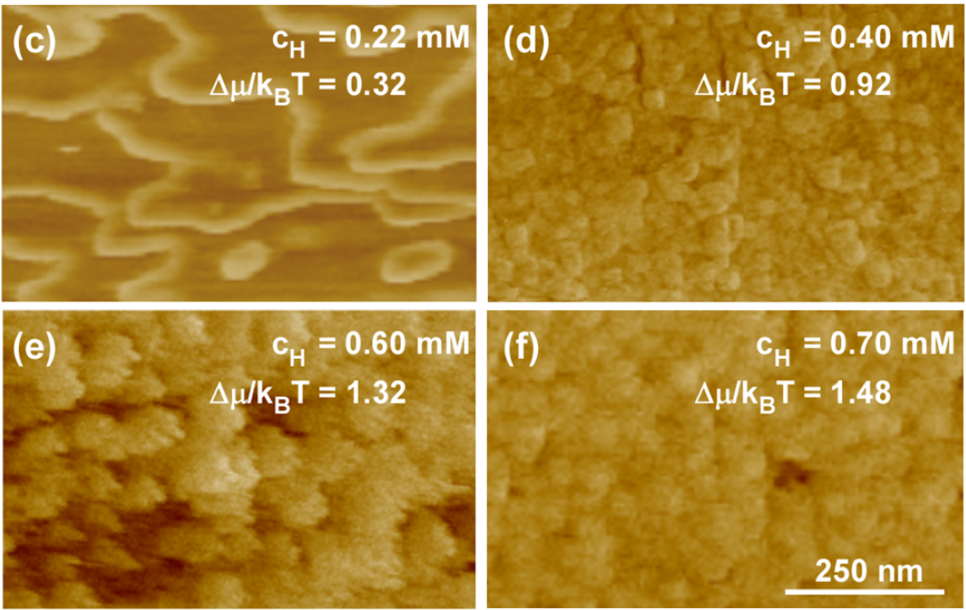
\includegraphics[width=\linewidth]{morfo_compara.png}\\
      \fig{Fig.~10. AFM en modo de fase a distintas sobresaturaciones (Olafson \emph{et al.}, 2017).}
    \end{column}
    \begin{column}{0.48\textwidth}
      \centering
      \setlength{\tabcolsep}{1pt}
      \begin{tabular}{@{}ccc@{}}
        \snap{0.155\textheight}{aniso_c_3.png} &
        \snap{0.155\textheight}{aniso_d_3.png} &
        \snap{0.155\textheight}{aniso_e_3.png} \\
        {\scriptsize $\sigma=0.38$} & {\scriptsize $\sigma=1.5$} & {\scriptsize $\sigma=2.7$}
      \end{tabular}\\
      \fig{Fig.~11. kMC 3D anisotrópico, $t=240$ min.}\\[0.4em]
      \begin{block}{\centering Misma fuerza impulsora}
        \centering\small
        $\Delta\mu/\kB T = \ln(1+\sigma) \approx 0.32,\ 0.92,\ 1.31$\\
        {\footnotesize $\leftrightarrow$ paneles AFM (c), (d), (e)}
      \end{block}
      {\footnotesize Acuerdo \textbf{cualitativo}: $\sigma\uparrow$ $\Rightarrow$ mayor densidad de núcleos}
    \end{column}
  \end{columns}
\end{frame}

% ---------------------------------------------------------------- 15: Conclusiones
\begin{frame}{Conclusiones}
  \begin{columns}[T,onlytextwidth]
    \begin{column}{0.56\textwidth}
      \begin{itemize}\setlength{\itemsep}{0.6em}
        \item \textbf{Modelo kMC 3D}: reproduce la cinética de conversión ($R^2=0.971$) y cualitativamente la morfología superficial.
        \item Transición de régimen con $\sigma$: islas lisas $\to$ superficie \textbf{rugosa}, en versiones isotrópica y anisotrópica.
        \item Energías de enlace \textbf{MACE} por dirección integradas satisfactoriamente al kMC anisotrópico.
      \end{itemize}
    \end{column}
    \begin{column}{0.40\textwidth}
      \begin{block}{Limitaciones}
        \small Morfología evaluada de forma cualitativa; ajuste cinético dependiente de parámetros estocásticos.
      \end{block}
      \vspace{0.3em}
      \begin{block}{Perspectivas}
        \small
        Parámetros de orden morfológicos\\[0.15em]
        Aceleración con \textit{transformers}\\[0.15em]
        Crecimiento con \textbf{antimaláricos}
      \end{block}
    \end{column}
  \end{columns}
\end{frame}

% ---------------------------------------------------------------- Cierre
\begin{frame}{¡Muchas gracias por su atención!}
  \vspace{0.4cm}
  \begin{center}
    \begin{minipage}{0.60\textwidth}
      \begin{block}{\centering Preguntas y Discusión}
        \centering\vspace{0.25cm}
        {\Large \textbf{¿Preguntas o comentarios?}}\\[0.25cm]
      \end{block}
    \end{minipage}
    
    \vspace{0.6cm}
    {\normalsize Código abierto: \texttt{github.com/SebastGg99/MalariaProject}}\\[0.25cm]
    {\scriptsize\color{gris}Agradecimientos: Proyecto Programática 2024-76972 · D.~Duque (cálculos MACE) · G.~Torres (código base)}
  \end{center}
\end{frame}

% =====================================================================
%  MATERIAL DE RESPALDO (Appendix)
% =====================================================================
\appendix

% ---------------------------------------------------------------- Respaldo Portadilla
\begin{frame}
  \vspace{1.2cm}
  \begin{center}
    {\usebeamerfont{title}\usebeamercolor[fg]{title}\huge\bfseries Material de Respaldo}\\[0.3cm]
    {\color{FisicaCyan}\rule{0.35\linewidth}{1.2pt}}
  \end{center}
\end{frame}

% ---------------------------------------------------------------- R1: Relajación
\begin{frame}{Relajación estructural del cristal}
  \framesubtitle{Dímero $\pi$--$\pi$ construido desde la estructura de Becker \emph{et al.} (2016), con PBC en 3D.}
  \begin{columns}[c,onlytextwidth]
    \begin{column}{0.48\textwidth}
      \begin{block}{Protocolo (ASE + MACE \textit{polar-1-l})}
        \footnotesize
        \textbf{1.} Solo celda: \texttt{StrainFilter} + L-BFGS\\
        \hspace*{1em}$F_{\max}=0.05$\,eV/\AA\\[0.3em]
        \textbf{2.} Celda + posiciones: \texttt{FrechetCellFilter} + L-BFGS\\
        \hspace*{1em}$F_{\max}=0.01$\,eV/\AA
      \end{block}
    \end{column}
    \begin{column}{0.48\textwidth}
      \centering\small
      \renewcommand{\arraystretch}{1.15}
      \begin{tabular}{@{}lcc@{}}
        \toprule
        Parámetro & Becker \emph{et al.} & \textbf{MACE} \\
        \midrule
        $a$ (\AA)           & 16.636  & \textbf{16.218} \\
        $b$ (\AA)           & 24.846  & \textbf{24.214} \\
        $c$ (\AA)           & 7.990   & \textbf{7.758} \\
        $\alpha$ ($^\circ$) & 135.205 & \textbf{135.440} \\
        $\beta$ ($^\circ$)  & 119.553 & \textbf{120.054} \\
        $\gamma$ ($^\circ$) & 36.874  & \textbf{37.008} \\
        \bottomrule
      \end{tabular}
    \end{column}
  \end{columns}
\end{frame}

% ---------------------------------------------------------------- R2: Red y PBC
\begin{frame}{Modelo kMC 3D sobre red}
  \framesubtitle{Red de $80\times80$ sitios de adsorción, vista desde arriba.}
  \vspace{-0.2cm}
  \begin{columns}[T,onlytextwidth]
    \begin{column}{0.32\textwidth}
      \centering
      \begin{tikzpicture}[x=0.33cm,y=0.33cm]
        \foreach \x in {0,...,4} \foreach \y in {0,...,4}
          \draw[gris!50,fill=white] (\x,\y) rectangle ++(1,1);
        \foreach \x/\y in {0/0,0/4,4/0,4/4,1/1,1/3,3/1,3/3}
          \node[font=\tiny,gris!60] at (\x+0.5,\y+0.5) {$\times$};
        \foreach \x/\y/\l in {2/3/N,2/1/S,3/2/E,1/2/W}{
          \fill[azul!45] (\x,\y) rectangle ++(1,1);
          \draw[white] (\x,\y) rectangle ++(1,1);
          \node[font=\scriptsize\bfseries,white] at (\x+0.5,\y+0.5) {\l};
        }
        \fill[acento] (2,2) rectangle ++(1,1);
        \draw[white] (2,2) rectangle ++(1,1);
      \end{tikzpicture}\\[0.2em]
      {\color{azul}\bfseries\small Vecindad de von Neumann}\par
    \end{column}
    \begin{column}{0.32\textwidth}
      \centering
      \begin{tikzpicture}[x=0.33cm,y=0.33cm,>=stealth]
        \foreach \y in {1,...,4}{
          \draw[dashed,gris!60,fill=acento!15] (5,\y) rectangle ++(1,1);
          \draw[dashed,gris!60,fill=azul!15] (0,\y) rectangle ++(1,1);
        }
        \foreach \x in {1,...,4} \foreach \y in {1,...,4}
          \draw[gris!60,fill=white] (\x,\y) rectangle ++(1,1);
        \foreach \y in {1,...,4}{
          \fill[acento!55] (1,\y) rectangle ++(1,1);
          \fill[azul!45] (4,\y) rectangle ++(1,1);
          \draw[white] (1,\y) rectangle ++(1,1);
          \draw[white] (4,\y) rectangle ++(1,1);
        }
        \draw[azul,thick] (1,1) rectangle (5,5);
        \draw[->,acento,thick] (1.5,5.1) to[out=35,in=145] node[above,font=\tiny,inner sep=1pt]{$x\equiv x+N$} (5.5,5.1);
      \end{tikzpicture}\\[0.2em]
      {\color{azul}\bfseries\small Fronteras periódicas}\par
    \end{column}
    \begin{column}{0.32\textwidth}
      \centering
      \begin{tikzpicture}[x=0.28cm,y=0.28cm]
        \foreach \row [count=\y] in {{1,1,1,2,2,2},{1,1,2,2,2,3},{1,1,2,2,3,3},{0,1,1,2,2,3},{0,0,1,1,2,2},{0,0,1,1,1,2}}{
          \foreach \h [count=\x] in \row {
            \pgfmathsetmacro{\pct}{12+24*\h}
            \ifnum\h>1 \def\tc{white}\else\def\tc{black}\fi
            \fill[azul!\pct] (\x,-\y) rectangle ++(1,1);
            \draw[white,line width=0.5pt] (\x,-\y) rectangle ++(1,1);
            \node[font=\tiny,text=\tc] at (\x+0.5,-\y+0.5) {\h};
          }
        }
      \end{tikzpicture}\\[0.2em]
      {\color{azul}\bfseries\small Mapa de alturas SOS (3D)}\par
    \end{column}
  \end{columns}
  \vspace{0.4em}
  \begin{center}
    \begin{minipage}{0.80\textwidth}
      \begin{block}{Modelo 3D adaptativo (\textit{solid-on-solid})}
        \footnotesize Adaptación de Nagpal \emph{et al.} (2024): adsorción dependiente de $\sigma$\\
        Aquí: \textbf{anisotropía} $E_{pb_x}\neq E_{pb_y}$ $+$ evento de \textbf{incorporación}
      \end{block}
    \end{minipage}
  \end{center}
\end{frame}

% ---------------------------------------------------------------- R3: Algoritmo kMC
\begin{frame}{Modelo 3D: selección y ejecución de eventos}
  \begin{columns}[c,onlytextwidth]
    \begin{column}{0.44\textwidth}
      \centering
      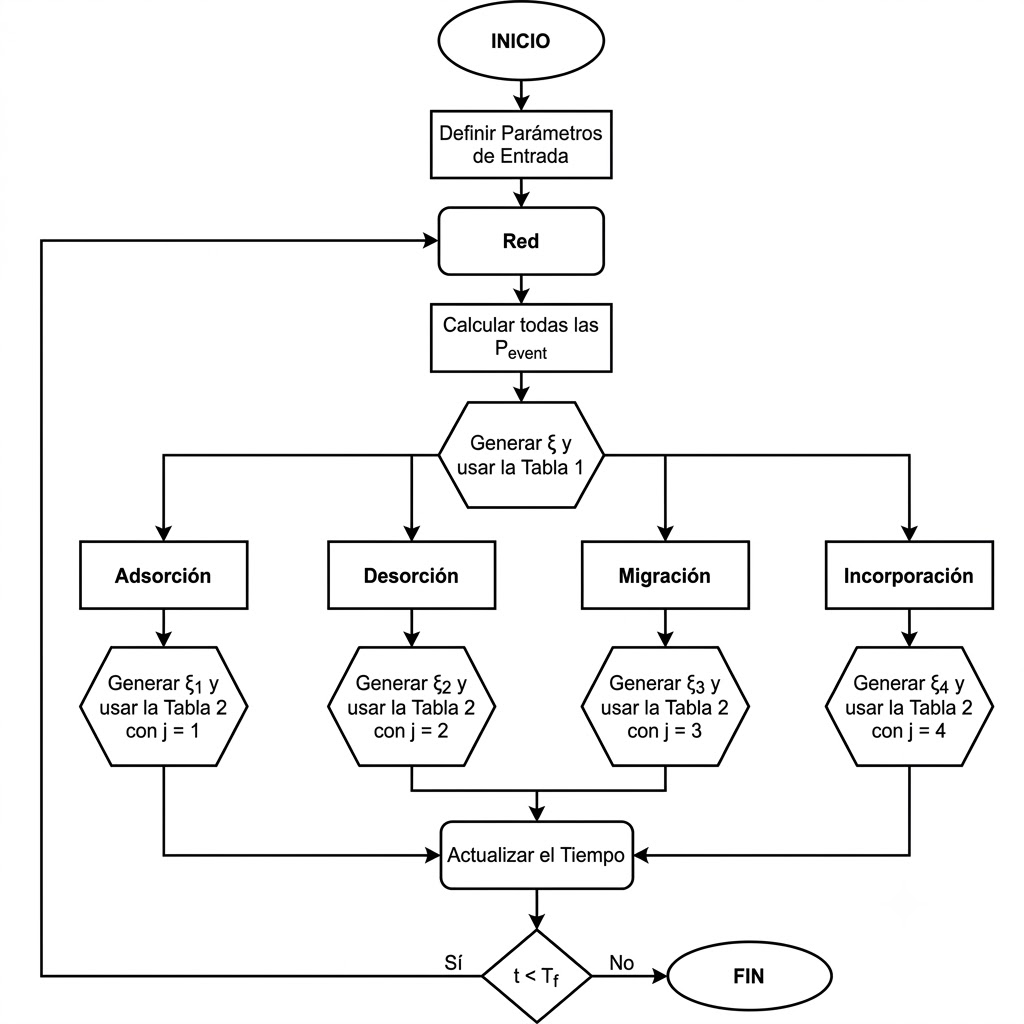
\includegraphics[height=0.60\textheight]{diagrama.png}\\
      \fig{Fig.~12. Diagrama de flujo del algoritmo kMC.}
    \end{column}
    \begin{column}{0.54\textwidth}
      \footnotesize
      {\color{azul}\bfseries Tabla 1.} Selección del evento ($P_j = W_j/W_{tot}$)\\[0.2em]
      \begin{tabular}{@{}ll@{}}
        \toprule
        $0<\zeta\le P_a$ & Adsorción \\
        $P_a<\zeta\le P_a+P_d$ & Desorción \\
        $P_a+P_d<\zeta\le P_a+P_d+P_m$ & Migración \\
        $P_a+P_d+P_m<\zeta\le 1$ & Incorporación \\
        \bottomrule
      \end{tabular}\\[0.8em]
      {\color{azul}\bfseries Tabla 2.} Selección de la clase $n$ (evento $j$)\\[0.2em]
      \renewcommand{\arraystretch}{1.2}\setlength{\tabcolsep}{3pt}
      \begin{tabular}{@{}ll@{}}
        \toprule
        $\dfrac{\sum_{m=0}^{n-1} r_j^{(m)}}{\sum_{m=0}^{4} r_j^{(m)}} < \zeta_j \le \dfrac{\sum_{m=0}^{n} r_j^{(m)}}{\sum_{m=0}^{4} r_j^{(m)}}$ & $n=0,\dots,4$ \\
        \bottomrule
      \end{tabular}\\[0.6em]
      Migración: dirección aleatoria; solo hacia un vecino \textbf{más bajo}.\\
      El tiempo avanza con la ec.~(14) aunque el evento no sea factible.
    \end{column}
  \end{columns}
\end{frame}

% ---------------------------------------------------------------- R4: Lisozima
\begin{frame}{Validación: lisozima (Nagpal \emph{et al.}, 2024)}
  \framesubtitle{Reproducción del modelo 3D isotrópico de referencia antes de aplicarlo a la hemozoína.}
  \begin{columns}[c,onlytextwidth]
    \begin{column}{0.36\textwidth}
      \centering
      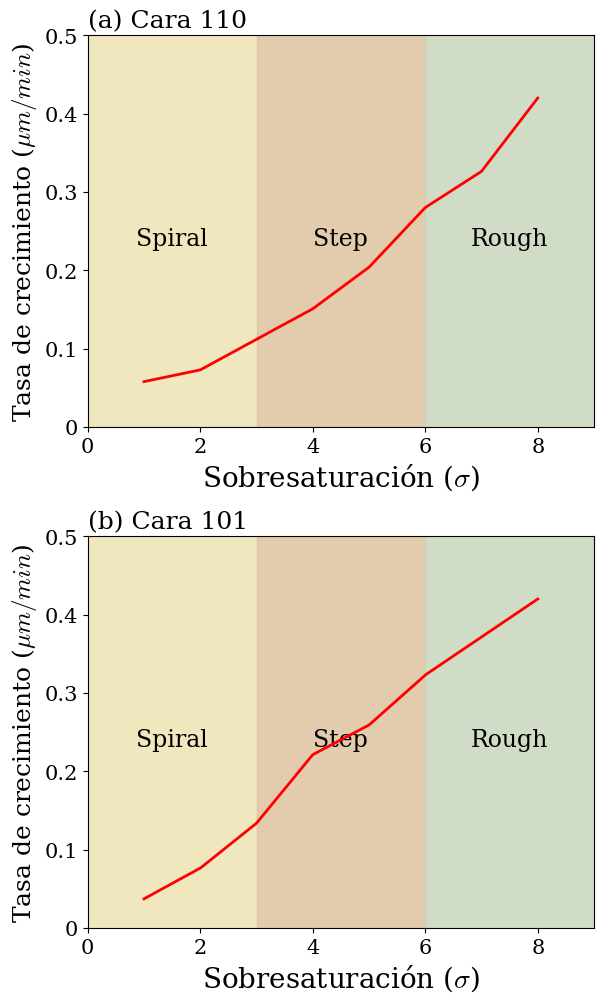
\includegraphics[height=0.55\textheight]{growth_rate_val.png}\\
      \fig{Fig.~13. Tasa de crecimiento vs.\ $\sigma$, caras (110) y (101).}
    \end{column}
    \begin{column}{0.62\textwidth}
      \centering
      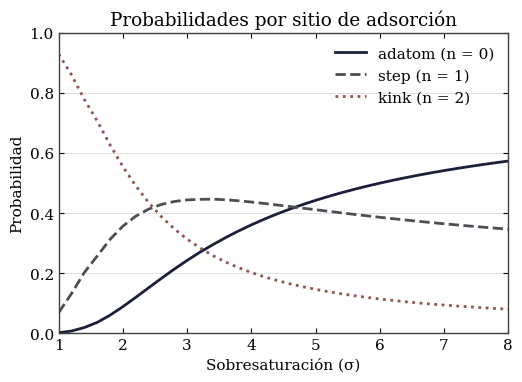
\includegraphics[width=0.64\linewidth]{PvsSite.png}\\
      \fig{Fig.~14. Probabilidad de adsorción por tipo de sitio vs.\ $\sigma$.}\\[0.3em]
      \begin{block}{\centering Lectura}
        \centering\small
        Cruces \textit{kink} $\to$ \textit{step} $\to$ adátomo \ $\Leftrightarrow$ \ espiral $\to$ escalón $\to$ rugoso
      \end{block}
    \end{column}
  \end{columns}
\end{frame}

% ---------------------------------------------------------------- R5: Morfología isotrópica
\begin{frame}{Resultados: morfología en el modelo 3D isotrópico}
  \begin{columns}[c,onlytextwidth]
    \begin{column}{0.70\textwidth}
      \centering
      \setlength{\tabcolsep}{1pt}
      \renewcommand{\arraystretch}{0.8}
      \begin{tabular}{@{}r@{\hspace{4pt}}ccc@{}}
        & {\scriptsize $t=30$ min} & {\scriptsize $t=60$ min} & {\scriptsize $t=240$ min} \\
        {\scriptsize $\sigma=0.38$} & \snap{0.185\textheight}{iso_c_1_1.png} & \snap{0.185\textheight}{iso_c_2.png} & \snap{0.185\textheight}{iso_c_3.png} \\
        {\scriptsize $\sigma=1.5$}  & \snap{0.185\textheight}{iso_d_1.png}   & \snap{0.185\textheight}{iso_d_2.png} & \snap{0.185\textheight}{iso_d_3.png} \\
        {\scriptsize $\sigma=2.7$}  & \snap{0.185\textheight}{iso_e_1.png}   & \snap{0.185\textheight}{iso_e_2.png} & \snap{0.185\textheight}{iso_e_3.png}
      \end{tabular}\\[0.1em]
      \fig{Fig.~15. Snapshots del modelo 3D isotrópico (red $80\times80$).}
    \end{column}
    \begin{column}{0.28\textwidth}
      \centering\scriptsize
      {\color{azul}\bfseries Optimización bayesiana}\\[0.2em]
      \renewcommand{\arraystretch}{1.1}
      \begin{tabular}{@{}lc@{}}
        \toprule
        $E_{pb}/\kB T$ & 1.27 \\
        $\phi/\kB T$   & 1.48 \\
        $\delta$       & 1.78 \\
        $K_0^{+}$      & 11.67 \\
        $K_{inc}^{+}$  & 0.507 \\
        \bottomrule
      \end{tabular}\\[0.6em]
      \begin{block}{\centering Lectura}
        \centering
        $\sigma\uparrow$ $\Rightarrow$ más núcleos, islas menos definidas $\Rightarrow$ \textbf{mayor rugosidad}
      \end{block}
    \end{column}
  \end{columns}
\end{frame}

\end{document}